\chapter{Experimentación y resultados}
\label{chap:experimentacion}

%% que resultados se obtienen

En este capítulo se presentan los resultados obtenidos a partir del procedimiento experimental descrito en el Capítulo~\ref{chap:metodologia_experimental}. El análisis se organiza de forma progresiva, comenzando por el comportamiento de las metaheurísticas consideradas y avanzando posteriormente hacia la evaluación de los modelos subrogados y su integración en el proceso de optimización.

En primer lugar, se analiza el comportamiento de AGE, DE y SHADE con el fin de identificar posibles fases de estancamiento y valorar el efecto del reinicio elitista sobre las trayectorias generadas. A continuación, se comparan las estrategias \textit{offline} de evaluación de modelos subrogados, se seleccionan las técnicas más prometedoras y se realiza su ajuste de hiperparámetros. Finalmente, se estudia la integración \textit{online} del modelo seleccionado dentro del bucle de optimización.


% ============================================================
\section{Estancamiento de las metaheurísticas y evaluación del reinicio elitista}
\label{sec:resultados_reinicio}
% ============================================================

En esta primera parte del análisis se estudia el comportamiento de AGE, DE y SHADE en ausencia de reinicio, con el objetivo de comprobar si sus trayectorias mantienen una dinámica suficientemente informativa durante todo el presupuesto de evaluaciones. Una vez identificado el problema de estancamiento, se evalúa el criterio de reinicio definido en el Capítulo~\ref{chap:algo_tecnicas_ref}.

Este análisis tiene un papel auxiliar dentro del trabajo: el objetivo principal no es optimizar el criterio de reinicio en sí mismo, sino evitar que las trayectorias utilizadas posteriormente para la evaluación de subrogados queden dominadas por fases largas de convergencia prematura. Por tanto, la finalidad no es comparar las metaheurísticas entre sí, sino determinar si cada una de ellas necesita un mecanismo de reactivación y qué ventana de estancamiento resulta aceptable para generar datos más útiles sin deteriorar de forma relevante la calidad final.


% ------------------------------------------------------------
\subsection{Motivación del reinicio}
\label{subsec:motivacion_reinicio}
% ------------------------------------------------------------


En ausencia de reinicio, la dinámica de cada metaheurística determina por completo la distribución de las muestras generadas. Cuando la búsqueda deja de producir mejoras relevantes antes de agotar dicho presupuesto, las evaluaciones posteriores tienden a concentrarse en torno a valores de \textit{fitness} muy similares, lo que reduce la variabilidad disponible para entrenar y validar modelos subrogados.

La Figura~\ref{fig:convergencia_sin_reinicio} muestra las curvas de convergencia promedio para tres funciones con características de paisaje diferentes. En \(f_1\), los algoritmos alcanzan rápidamente una zona estable; en \(f_{10}\), el comportamiento es más gradual, pero también aparecen tramos prolongados con poca mejora; finalmente, en \(f_{29}\), las curvas presentan una caída inicial casi instantánea seguida de una evolución prácticamente plana. Con estos ejemplos se verifica como gran parte relevante de la trayectoria generada por una metaheurística puede quedar dominada por fases de mejora muy reducida o incluso inexistentes.

La consecuencia directa de este estancamiento sobre la calidad de los datos generados se aprecia al analizar la distribución del error por bloques temporales. La Figura~\ref{fig:bloques_sin_reinicio} divide el presupuesto en cinco bloques del 20\% y muestra la distribución del error logarítmico en cada uno de ellos para una función representativa.

Como se observa en la figura, los primeros bloques presentan una distribución amplia que cubre distintas regiones del espacio de búsqueda. Sin embargo, a medida que aumenta el número de evaluaciones, las muestras se concentran progresivamente en un rango estrecho de valores. Desde la perspectiva del aprendizaje subrogado, estas muestras tardías son menos discriminativas, ya que el modelo recibe evaluaciones muy similares entre sí y dispone de menos información para distinguir soluciones de distinta calidad.

\begin{figure}[H]
    \centering
    \begin{subfigure}[t]{0.8\textwidth}
        \centering
        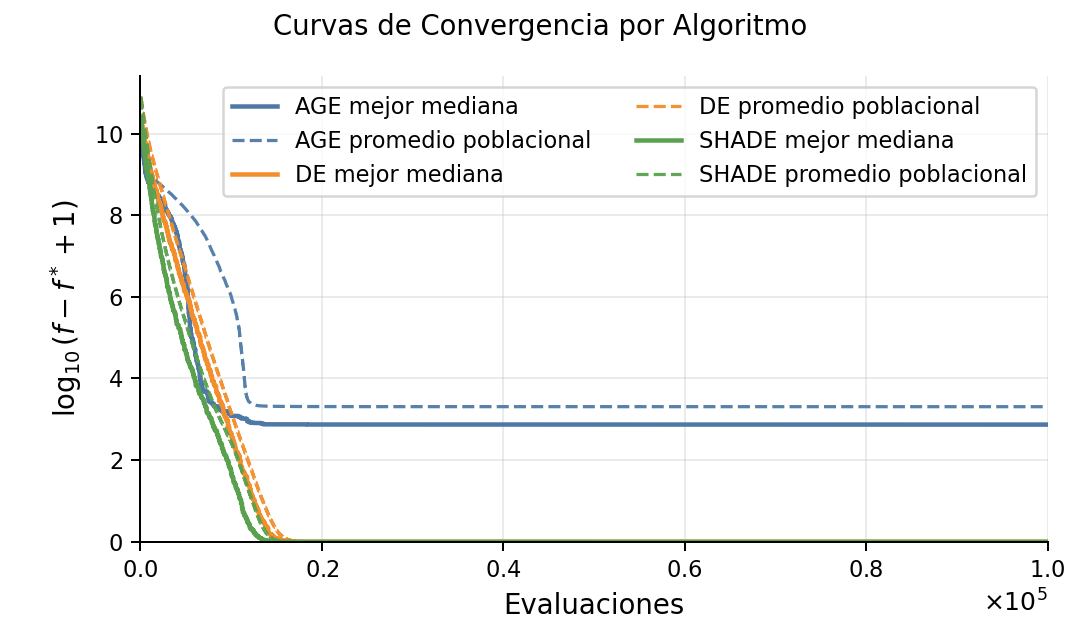
\includegraphics[width=\textwidth]{figuras/plots_sin_reinicio/curva_convergencia_cec2017_f1.png}
        \caption{\(f_1\)}
        \label{fig:convergencia_sin_reinicio_f1}
    \end{subfigure}
    \hfill
    \begin{subfigure}[t]{0.8\textwidth}
        \centering
        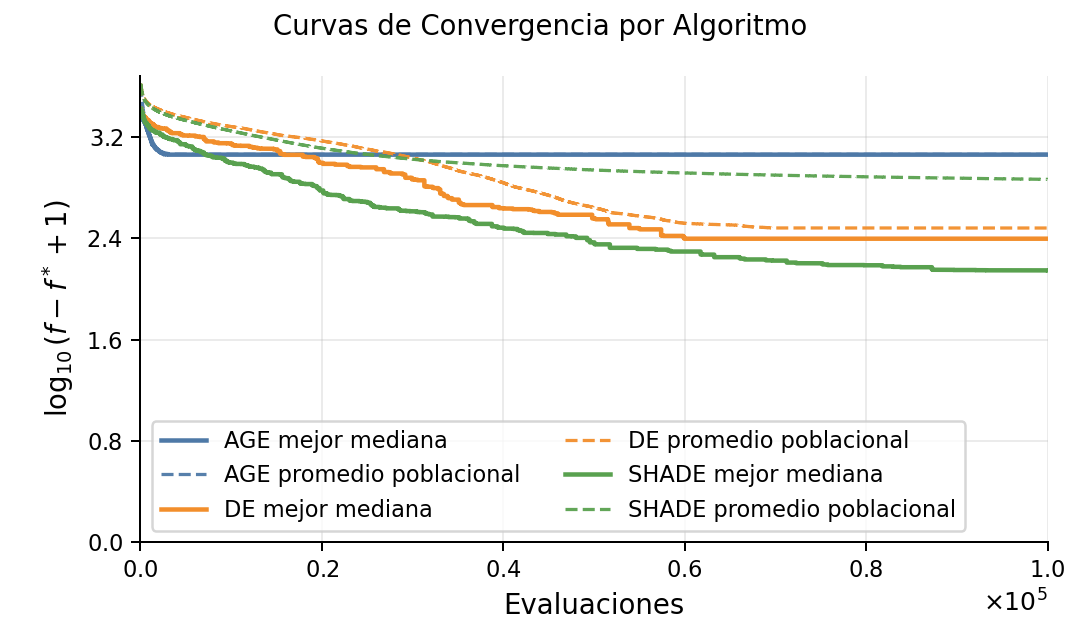
\includegraphics[width=\textwidth]{figuras/plots_sin_reinicio/curva_convergencia_cec2017_f10.png}
        \caption{\(f_{10}\)}
        \label{fig:convergencia_sin_reinicio_f10}
    \end{subfigure}

    \vspace{0.4cm}

    \begin{subfigure}[t]{0.8\textwidth}
        \centering
        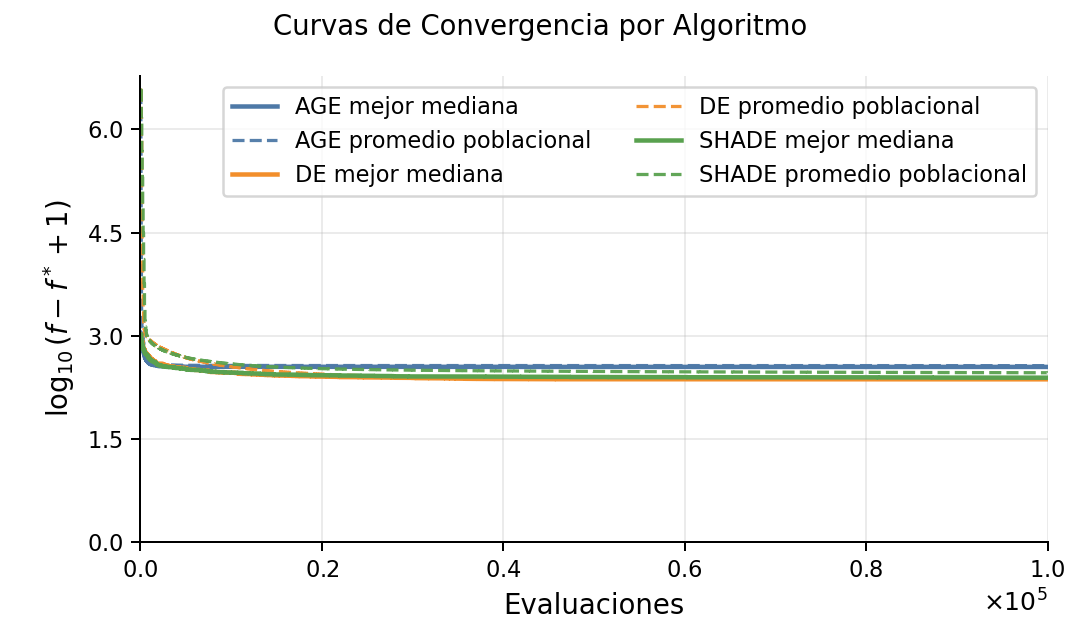
\includegraphics[width=\textwidth]{figuras/plots_sin_reinicio/curva_convergencia_cec2017_f29.png}
        \caption{\(f_{29}\)}
        \label{fig:convergencia_sin_reinicio_f29}
    \end{subfigure}
    \caption{Curvas de convergencia promedio sin reinicio en tres funciones representativas de CEC2017.}
    \label{fig:convergencia_sin_reinicio}
\end{figure}

\begin{figure}[H]
    \centering
    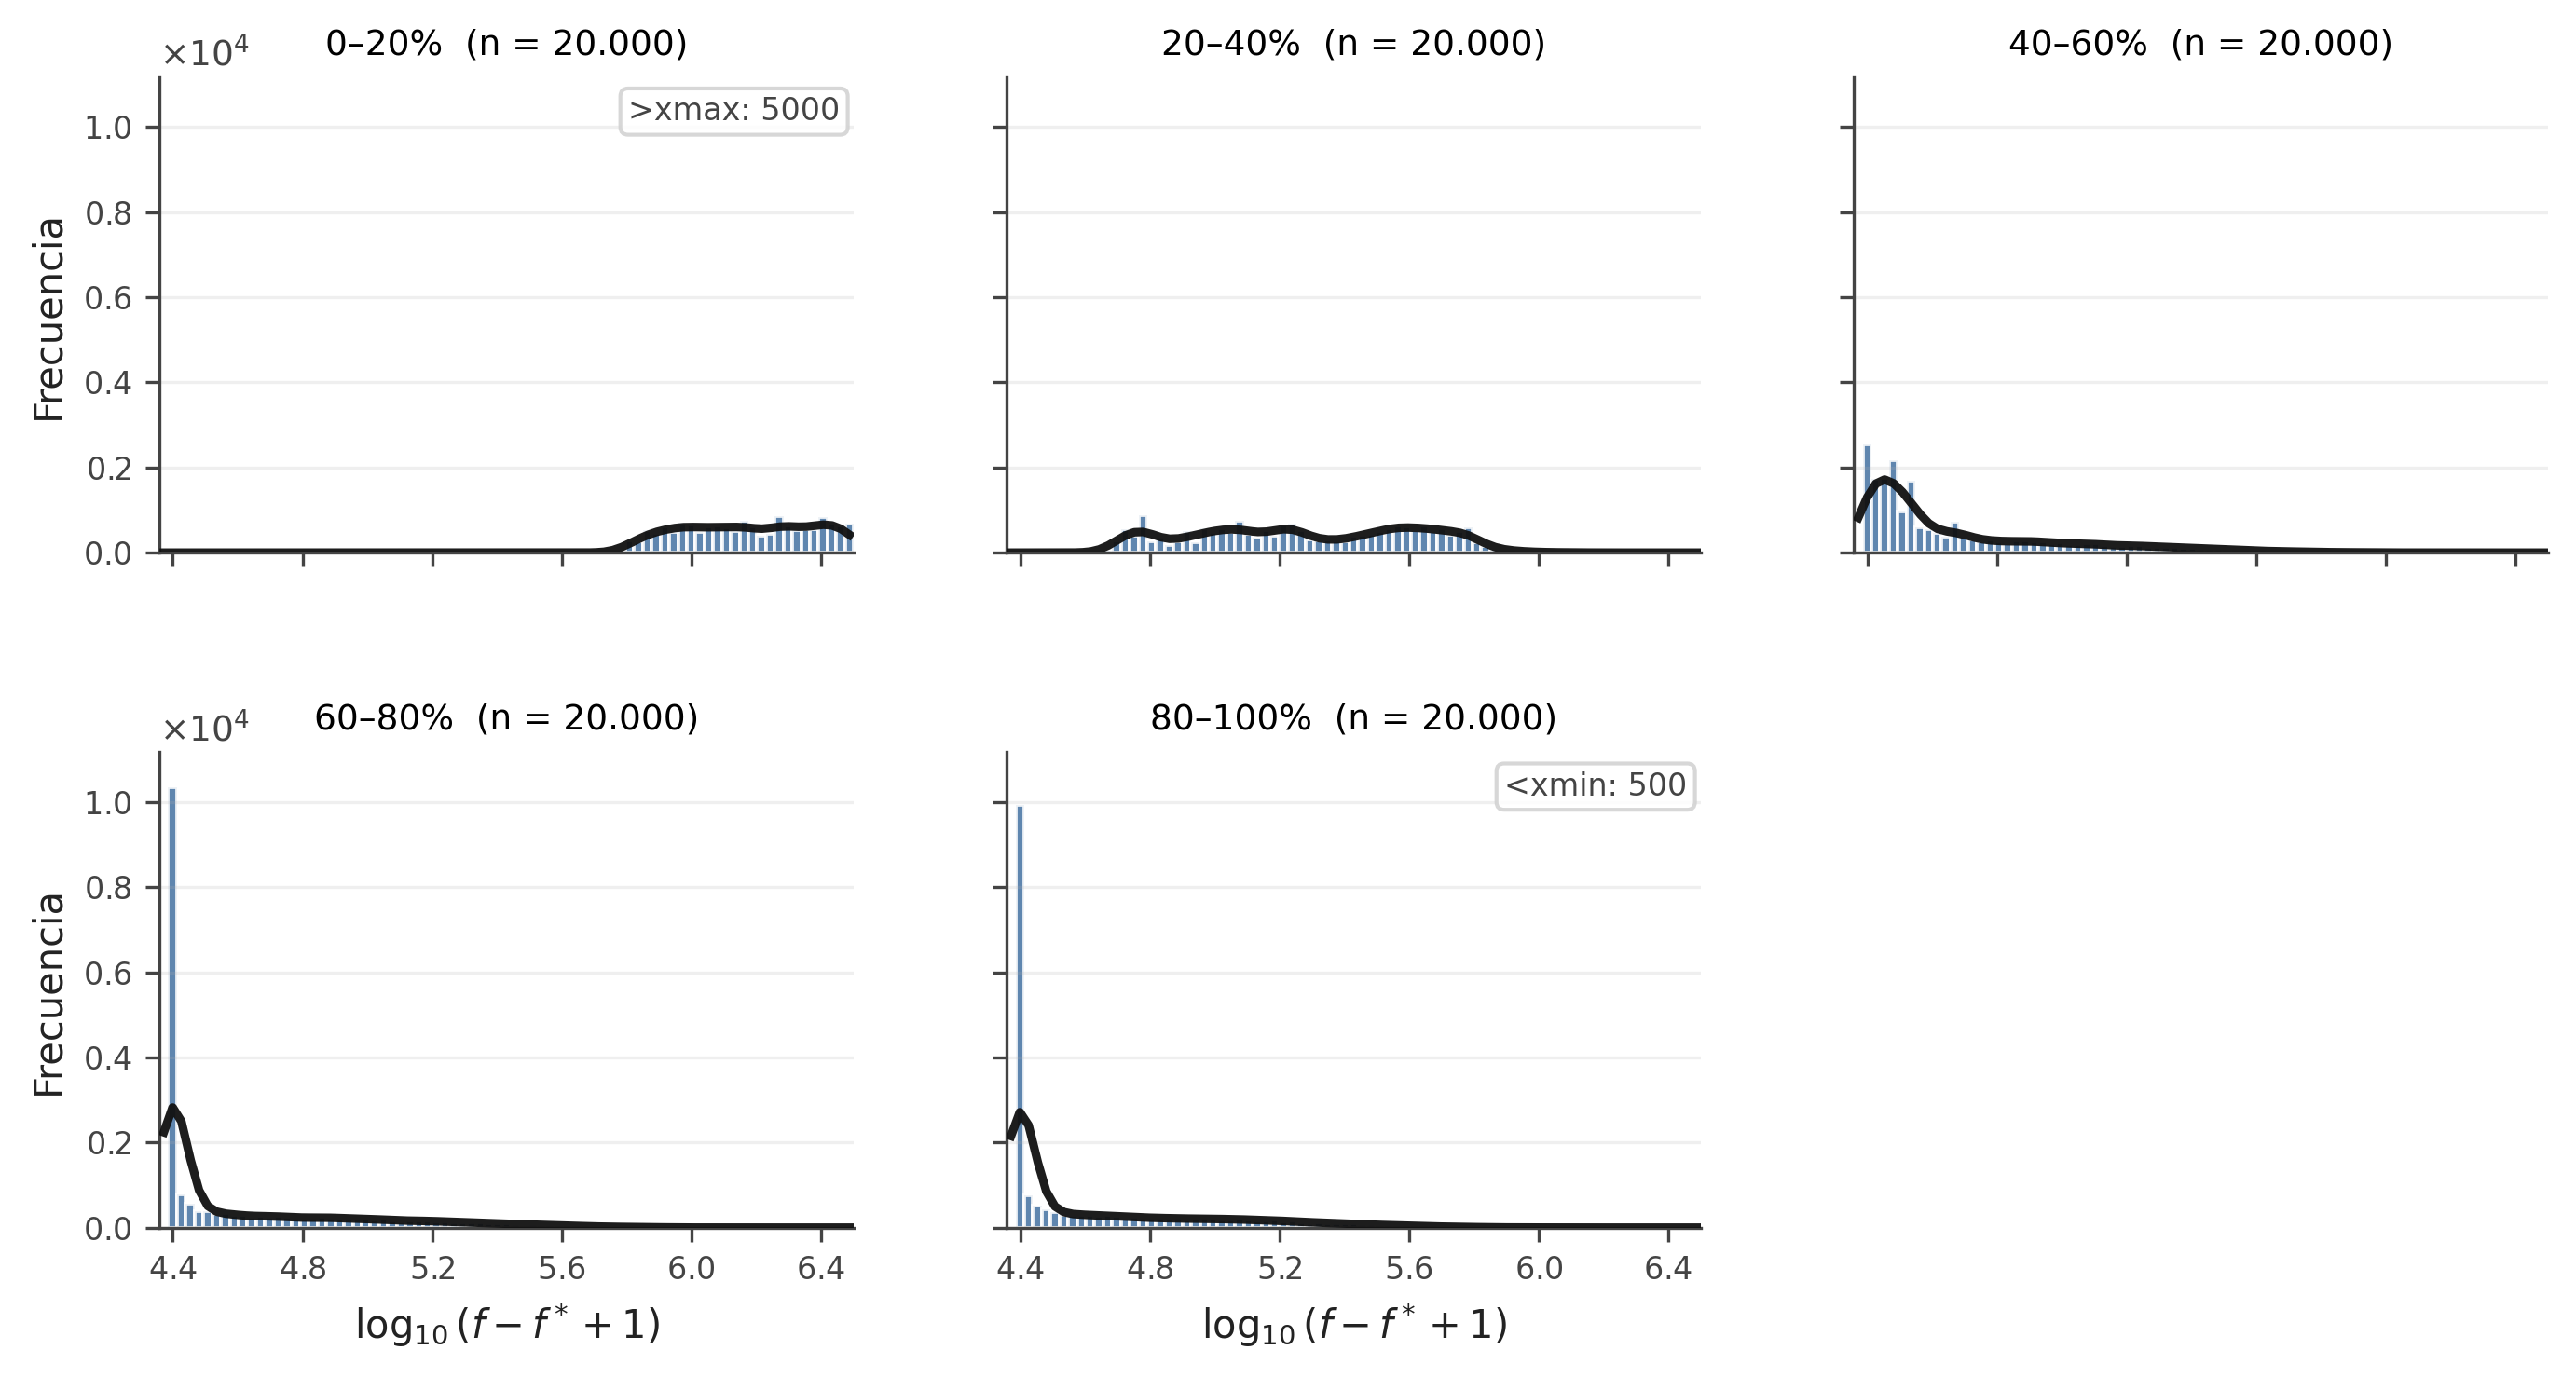
\includegraphics[width=1.0\textwidth]{figuras/plots_sin_reinicio/por_run/f12/age/sin_reinicio/histograma_fitness_fases_cec2017_f12_s41_sin_reinicio_age.png}
    \caption{Convergencia progresiva del error evaluada por bloques de la trayectoria: AGE sobre \(f_{12}\) (semilla 41).}
    \label{fig:bloques_sin_reinicio}
\end{figure}


Para evitar que las trayectorias queden dominadas por estas fases de estancamiento, se incorpora el criterio de reinicio elitista descrito en el Capítulo~\ref{chap:algo_tecnicas_ref}. A continuación, se evalúan las distintas configuraciones propuestas en el Capítulo~\ref{chap:metodologia_experimental} de dicho criterio con el objetivo de identificar, para cada metaheurística, aquella que mejor equilibre la reactivación de la búsqueda con la preservación de la calidad final de las soluciones.


% ------------------------------------------------------------
\subsection{Evaluación de las configuraciones de reinicio}
\label{subsec:evaluacion_reinicio}
% ------------------------------------------------------------

Una vez visualizado el problema del estancamiento, el objetivo no es establecer una clasificación global entre AGE, DE y SHADE, sino determinar si alguna configuración con reinicio resulta adecuada para generar las trayectorias que utilizarán posteriormente los modelos subrogados en las estrategias \textit{offline} y \textit{online}. En particular, se busca una configuración que reduzca el estancamiento sin introducir deterioros importantes en la calidad final.

Como punto de partida, se analiza si es posible seleccionar una única ventana de estancamiento común para las tres metaheurísticas. Adoptar una configuración global reduciría el riesgo de ajustar el criterio de reinicio de forma específica a un algoritmo concreto o al propio banco de problemas CEC2017. Para ello, se comparan las configuraciones definidas en el
Capítulo~\ref{chap:metodologia_experimental}: ventanas del \(1\%\), \(3\%\),
\(5\%\), \(7\%\) y \(10\%\) del presupuesto total de evaluaciones, junto con la versión sin reinicio.

Para cada metaheurística se consideran cuatro configuraciones:

\begin{table}[H]
    \centering
    \begin{tabular}{llc}
        \toprule
        \textbf{Configuración} & \textbf{Descripción}       & \textbf{Ventana de estancamiento} \\
        \midrule
        ALG                    & Sin reinicio               & --                                \\
        ALG-1                  & Reinicio con \(\rho=0.01\) & 1.000 evaluaciones                \\
        ALG-3                  & Reinicio con \(\rho=0.03\) & 3.000 evaluaciones                \\
        ALG-5                  & Reinicio con \(\rho=0.05\) & 5.000 evaluaciones                \\
        ALG-7                  & Reinicio con \(\rho=0.07\) & 7.000 evaluaciones                \\
        ALG-10                 & Reinicio con \(\rho=0.10\) & 10.000 evaluaciones               \\
        \bottomrule
    \end{tabular}
    \caption[Configuraciones genéricas de reinicio consideradas para cada metaheurística.]{Configuraciones genéricas de reinicio consideradas para cada metaheurística, donde \textbf{ALG} representa AGE, DE o SHADE.}
    \label{tab:configuraciones_reinicio_genericas}
\end{table}

Antes de analizar el impacto del reinicio, conviene evaluar empíricamente la agresividad del mecanismo. La Figura~\ref{fig:barplot_reinicios} muestra el número medio de reinicios activados por ejecución para cada configuración y metaheurística. Como era esperable, las ventanas de estancamiento menores provocan una activación más frecuente del mecanismo, por lo que esta información ayuda a interpretar los resultados posteriores sin sustituir a las comparaciones de calidad final.

\begin{figure}[htbp]
    \centering
    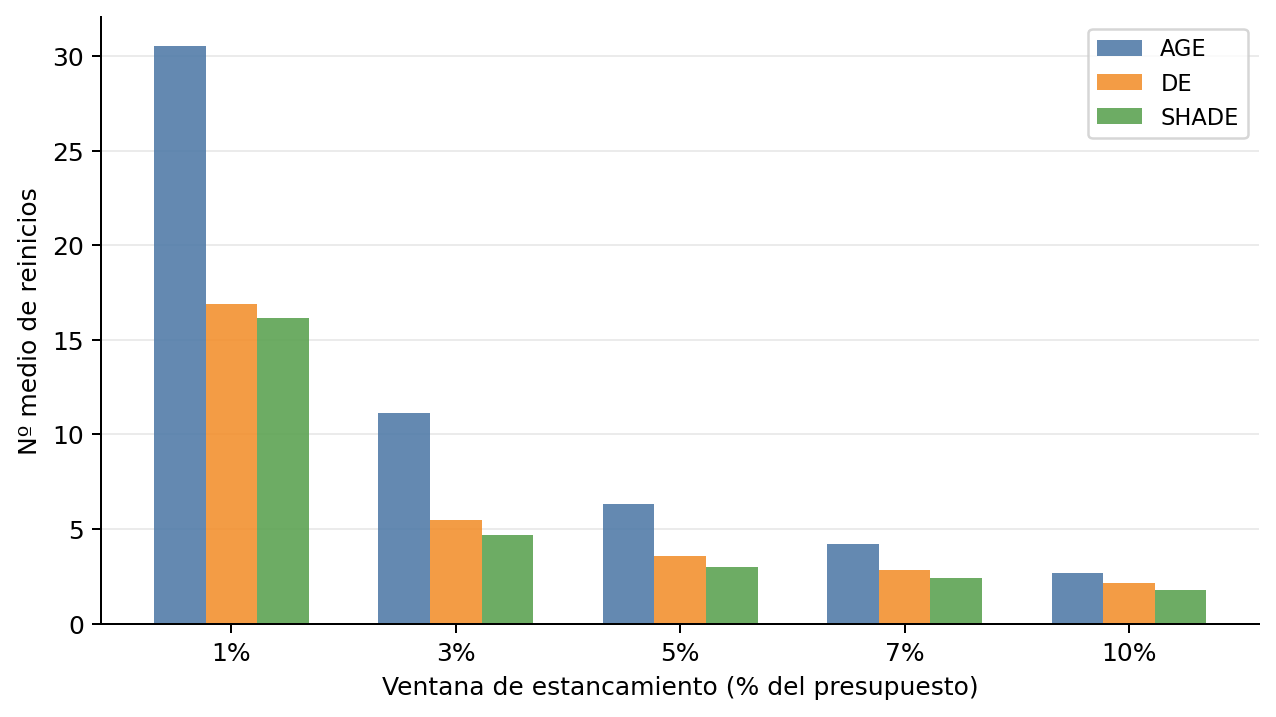
\includegraphics[width=0.9\textwidth]{figuras/barplot_reinicios_por_ventana_estancamiento.png}
    \caption{Número medio de reinicios elitistas por ejecución según la ventana de estancamiento \(\rho\).}
    \label{fig:barplot_reinicios}
\end{figure}

La selección final se apoya en las comparaciones de rendimiento generadas con
\textbf{TACOLAB}. Siguiendo el criterio metodológico definido en la
Sección~\ref{subsec:criterio_comparacion_modelos}, se prioriza el ranking medio calculado por TACOLAB, que permite resumir la posición relativa de cada
configuración sobre funciones con escalas de error heterogéneas. Las medias
del error final, recogidas en el Apéndice~\ref{ap:tablas_tacolab_reinicio}, se utilizan como apoyo complementario para comprobar que la configuración
seleccionada no introduce deterioros relevantes frente a la versión sin
reinicio.

Para estudiar esta evolución a lo largo de la ejecución, las Tablas~\ref{tab:ranking_reinicio_age}, \ref{tab:ranking_reinicio_de} y \ref{tab:ranking_reinicio_shade} muestran los rankings medios en distintos hitos del presupuesto de evaluaciones, siendo el 100\% el de mayor interés.

\begin{table}[H]
    \centering
    \footnotesize
    \setlength{\tabcolsep}{6pt}
    \renewcommand{\arraystretch}{0.95}
    \begin{tabular}{lccccc}
\toprule
\textbf{Configuración} & \multicolumn{5}{c}{\textbf{\% de evaluaciones}} \\
\cmidrule(lr){2-6}
{} & \textbf{20} & \textbf{40} & \textbf{60} & \textbf{80} & \textbf{100} \\
\midrule
AGE & 4.350 & 5.283 & 5.283 & 5.550 & 4.667 \\
AGE-1 & \textbf{1.783} & \textbf{1.350} & \textbf{1.600} & \textbf{1.333} & \textbf{1.600} \\
AGE-3 & 3.100 & 2.267 & 2.583 & 2.083 & 2.650 \\
AGE-5 & 3.517 & 3.667 & 3.400 & 3.350 & 3.367 \\
AGE-7 & 3.817 & 3.833 & 3.517 & 3.867 & 3.817 \\
AGE-10 & 4.433 & 4.600 & 4.617 & 4.817 & 4.900 \\
\bottomrule
\end{tabular}

    \caption{Ranking medio de TACOLAB para AGE en distintos hitos del presupuesto de evaluaciones.}
    \label{tab:ranking_reinicio_age}
\end{table}

\begin{table}[H]
    \centering
    \footnotesize
    \setlength{\tabcolsep}{6pt}
    \renewcommand{\arraystretch}{0.95}
    \begin{tabular}{lc}
\toprule
\textbf{Configuración} & \textbf{Rank medio (100\%)} \\
\midrule
DE-10 & \textbf{2.517} \\
DE-7 & 3.050 \\
DE-5 & 3.283 \\
DE-3 & 3.583 \\
DE & 4.017 \\
DE-1 & 4.550 \\
\bottomrule
\end{tabular}

    \caption{Ranking medio de TACOLAB para DE en distintos hitos del presupuesto de evaluaciones.}
    \label{tab:ranking_reinicio_de}
\end{table}

\begin{table}[H]
    \centering
    \footnotesize
    \setlength{\tabcolsep}{6pt}
    \renewcommand{\arraystretch}{0.95}
    \begin{tabular}{lccccc}
\toprule
\textbf{Configuración} & \multicolumn{5}{c}{\textbf{\% de evaluaciones}} \\
\cmidrule(lr){2-6}
{} & \textbf{20} & \textbf{40} & \textbf{60} & \textbf{80} & \textbf{100} \\
\midrule
SHADE & 3.200 & 3.083 & 3.033 & 3.267 & 3.550 \\
SHADE-1 & 4.600 & 4.450 & 4.517 & 4.583 & 4.583 \\
SHADE-3 & 4.000 & 3.917 & 3.883 & 3.750 & 3.717 \\
SHADE-5 & 3.183 & 3.633 & 3.583 & 3.450 & 3.283 \\
SHADE-7 & \textbf{2.883} & 3.167 & 3.250 & 3.117 & 2.950 \\
SHADE-10 & 3.133 & \textbf{2.750} & \textbf{2.733} & \textbf{2.833} & \textbf{2.917} \\
\bottomrule
\end{tabular}

    \caption{Ranking medio de TACOLAB para SHADE en distintos hitos del presupuesto de evaluaciones.}
    \label{tab:ranking_reinicio_shade}
\end{table}

El análisis de estos datos revela que el impacto del reinicio y la ventana evaluada no es uniforme entre los distintos algoritmos. Para aquellas ventanas muy pequeñas, correspondientes al 1\% y 3\% del presupuesto, se produce un escenario de reactivación muy frecuente donde, para un algoritmo como AGE, esta regeneración constante resulta adecuada, siendo AGE-1 la clara ganadora en la comparación por media final, con el mejor resultado en 25 de las 30 funciones y obteniendo el mejor ranking en todos los hitos. En cambio, este mismo patrón no se reproduce en DE ni en SHADE (véase en la Figura~\ref{fig:reinicio_shade_f10}). Las configuraciones con ventanas del 1\% se colocan en los peores puestos desde el inicio al ser ser metaheurísticas que requieren un mayor margen de evaluaciones para explotar la información acumulada en la población antes de que resulte conveniente reactivar la búsqueda (véase en la Figura~\ref{fig:convergencia_sin_reinicio}).

A medida que aumenta la ventana de estancamiento, el comportamiento cambia y las mejoras y empeoramientos vistos en las ventanas anteriores se pronuncian aún más. En DE y SHADE, las ventanas largas permiten preservar durante más tiempo la dinámica de búsqueda y conducen a los mejores rankings finales, especialmente con la configuración del 10\%. Por el contrario, en AGE una ventana tan amplia ralentiza su capacidad de respuesta, donde AGE-10 obtiene incluso un peor ranking final que la variante sin reinicio. Por tanto, no existe una ventana óptima común para las tres metaheurísticas ya que la configuración adecuada depende de la dinámica de búsqueda propia de cada algoritmo.

Esta clara diferencia de necesidades se refleja visualmente en la Figura~\ref{fig:rendimiento_agregado_malla}, que confirma el análisis extraído de las tablas comparativas: la curva de AGE se deteriora a medida que la ventana se hace más grande, mientras que las trayectorias de DE y SHADE mejoran progresivamente hasta alcanzar su punto óptimo en los valores más altos.

\begin{figure}[htbp]
    \centering
    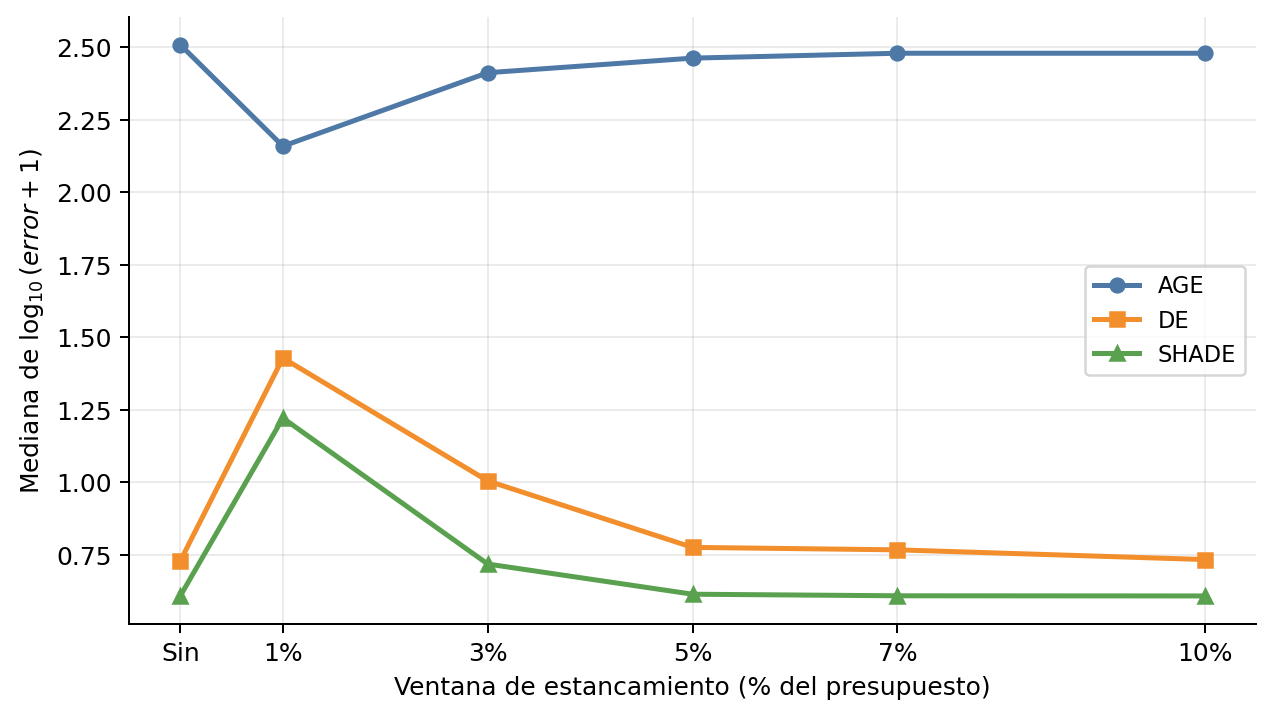
\includegraphics[width=0.95\textwidth]{figuras/rendimiento_por_ventana_estancamiento.png}
    \caption{Evolución del rendimiento agregado en función del tamaño de la ventana de estancamiento \(\rho\).}
    \label{fig:rendimiento_agregado_malla}
\end{figure}

\begin{figure}[htbp]
    \centering
    \begin{subfigure}{0.95\textwidth}
        \centering
        
\includegraphics[width=\textwidth]{figuras/reinicio/curva_convergencia_reinicio_cec2017_f10_shade.png}
        \caption{Convergencia}
    \end{subfigure}
    \hfill
    \begin{subfigure}{0.95\textwidth}
        \centering
        
\includegraphics[width=\textwidth]{figuras/reinicio/curva_diversidad_reinicio_cec2017_f10_shade.png}
        \caption{Diversidad}
    \end{subfigure}
    \caption{Ejemplo de reinicio en SHADE sobre \(f_{10}\) con \(\rho=0.01\).}
    \label{fig:reinicio_shade_f10}
\end{figure}



% ============================================================
\subsection{Conclusiones sobre la reactivación de la búsqueda}
\label{subsec:conclusiones_reinicio_parcial}
% ============================================================

%% deberiamos decidir en esta si se usa ventana común o específica, justificandolo con los resultados.

%% si finalmente elegimos ventanas distintas, tenemos que explicarlo como una excepcion motivada por los datos, no como punto de partida.

A partir del análisis anterior, los resultados dejan claro que es inviable utilizar una única ventana de estancamiento común para todas las metaheurísticas.

Por tanto, las configuraciones más adecuadas para cada algoritmo son:

\begin{table}[H]
    \centering
    \small
    \begin{tabular}{lc}
        \toprule
        \textbf{Algoritmo} & \textbf{Configuración} \\
        \midrule
        AGE                & AGE-1                  \\
        DE                 & DE-10                  \\
        SHADE              & SHADE-10               \\
        \bottomrule
    \end{tabular}
    \caption{Configuraciones seleccionadas para la generación de trayectorias en la fase de subrogados.}
    \label{tab:configuraciones_reinicio_seleccionadas}
\end{table}

Con las configuraciones fijadas, la siguiente fase evalúa las estrategias de entrenamiento \textit{offline} de los modelos subrogados sobre trayectorias menos dominadas por estancamiento y, por tanto, más adecuadas para analizar la capacidad predictiva de los modelos.

\section{Estudio offline: técnicas \textit{subrogadas} y configuración de entrenamiento}
\label{sec:estudio_offline}

% Siguiendo el protocolo descrito en la
% Sección~\ref{subsec:funciones_cribado_offline}, la comparativa inicial se
% realiza sobre el subconjunto representativo de funciones seleccionado para
% la fase de cribado.

Esta sección tiene como objetivo determinar empíricamente qué combinación de modelo subrogado y estrategia de entrenamiento ofrece el mejor compromiso entre fidelidad ordinal, precisión métrica y eficiencia computacional. Para ello, se comparan de forma \textit{offline} las técnicas consideradas y las estructuras de aprendizaje definidas en el Capítulo \ref{chap:algo_tecnicas_ref}, utilizando para el entrenamiento las trayectorias históricas generadas por las configuraciones finales de las metaheurísticas seleccionadas.

Siguiendo el protocolo definido en la
Subsección~\ref{subsec:funciones_cribado_offline}, la comparación inicial de modelos se realiza sobre el subconjunto representativo de funciones seleccionado para el cribado \textit{offline}, manteniendo las \(51\) semillas empleadas en la generación de trayectorias.

\subsection{Viabilidad Computacional y Estrategia Global}
\label{subsec:viabilidad_estrategia_global}

De cara a la futura integración \textit{online}, el coste computacional es muy relevante, especialmente el \textbf{tiempo de entrenamiento y predicción}. En este sentido, al llevar a cabo la ejecución de los distintos modelos de Aprendizaje Automático aplicados como técnicas de subrogado, el modelo \textit{Support Vector Regression} (SVR) evidenció limitaciones significativas dependiendo de la estrategia de entrenamiento empleada.

Mientras que el volumen de datos se mantiene constante en bloques fijos del 20 \% del presupuesto para la estrategia no acumulativa, mantener un historial de muestras cuyo tamaño incrementa en cada paso cronológico como conjunto de entrenamiento descarta a SVR de la estrategia acumulativa. Al escalar su complejidad de forma no lineal ($\mathcal{O}(N^3)$) respecto al número de muestras, el tiempo de ejecución se volvió desconsiderado para cualquier función (vease en la Figura \ref{fig:viabilidad_svr_f4}).

\begin{figure}[htbp]
    \centering
    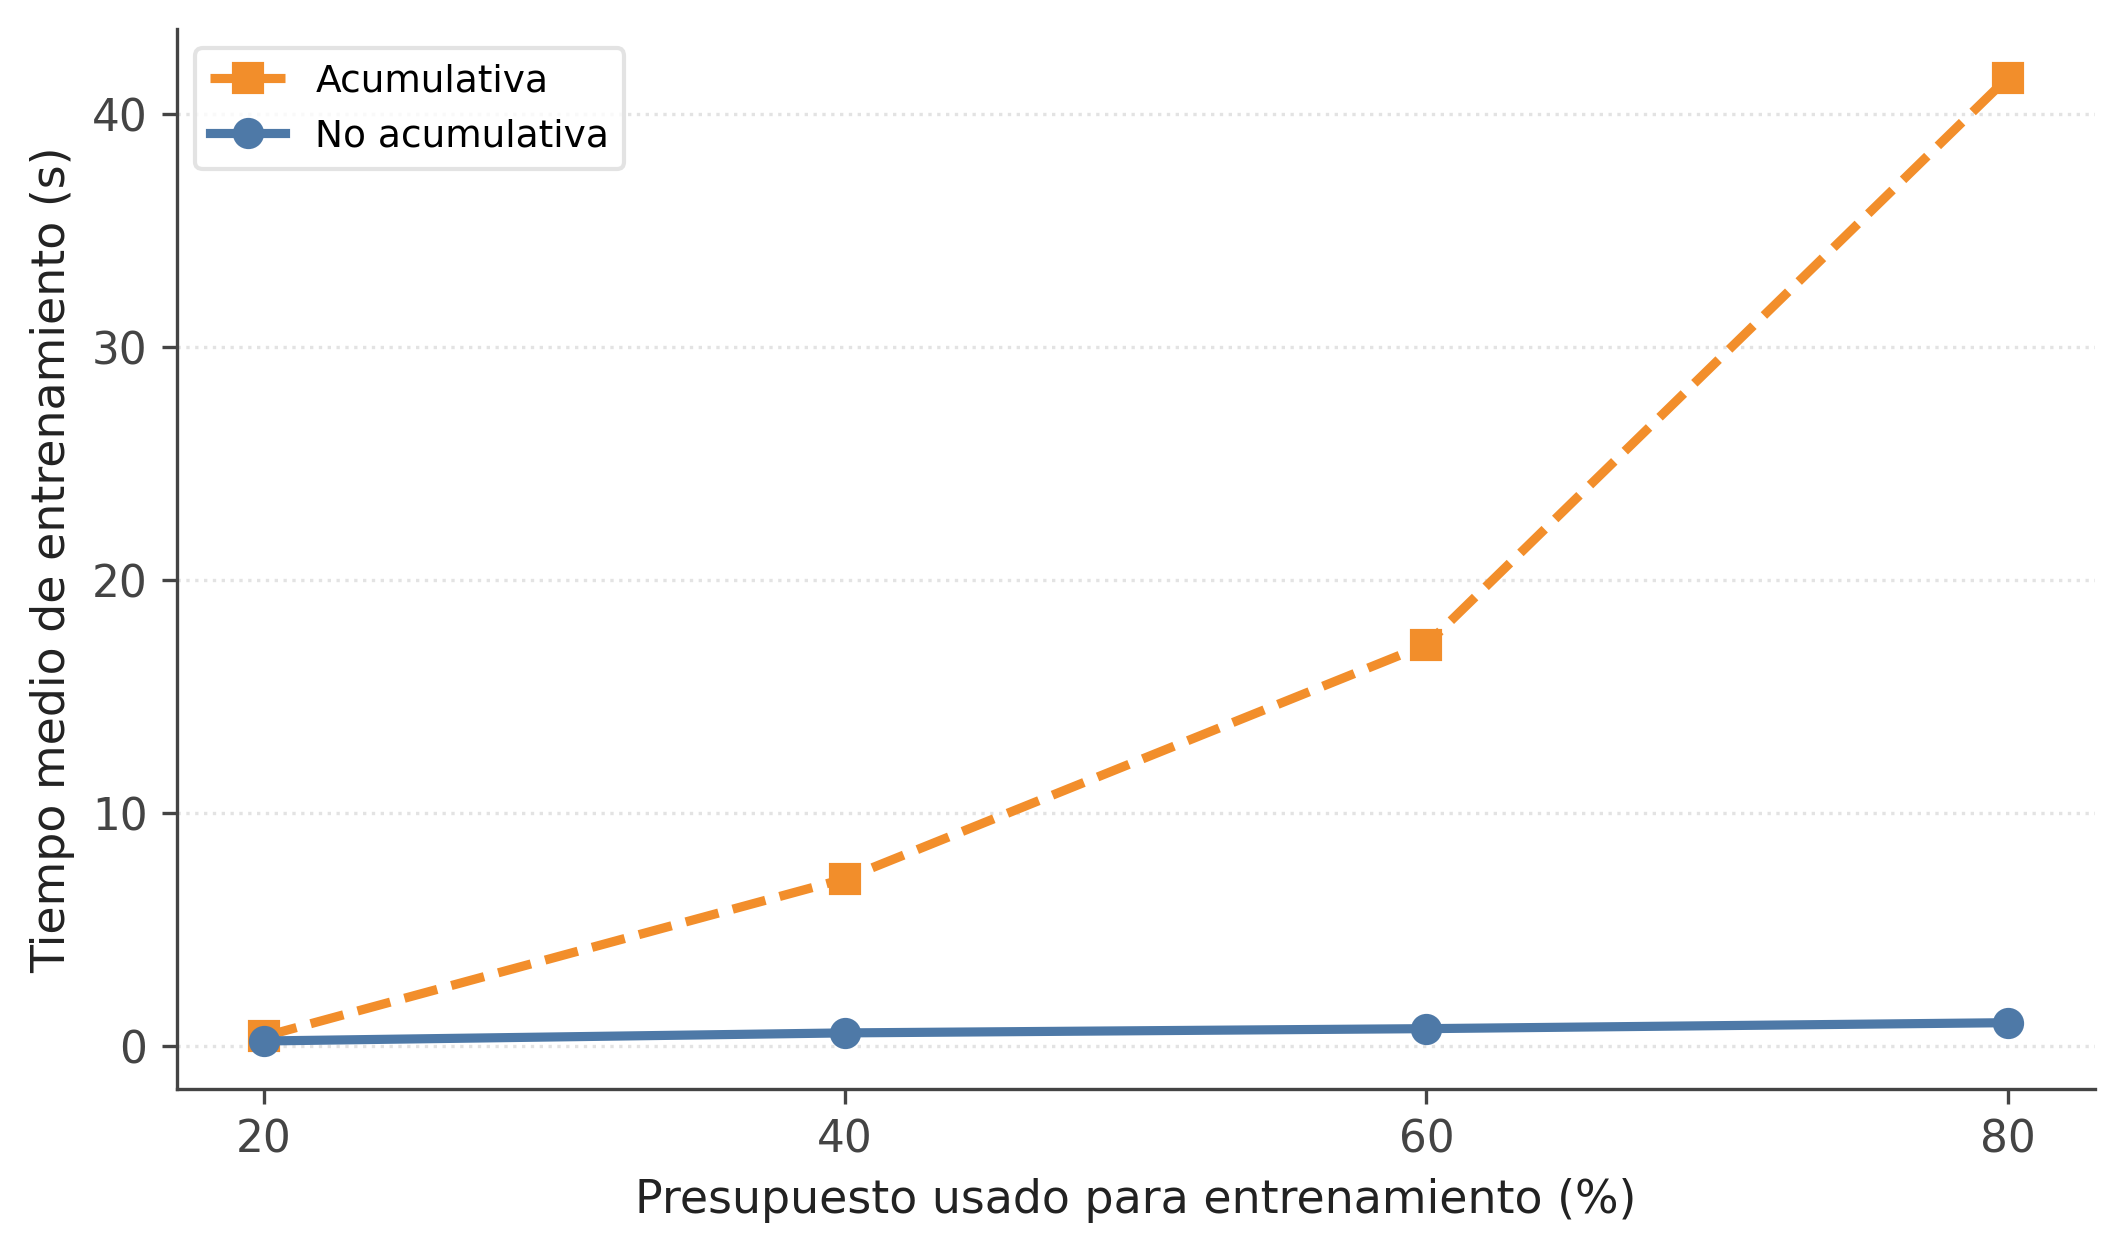
\includegraphics[width=0.9\textwidth]{figuras/surrogates_offline/viabilidad_svr_tiempo_entrenamiento_f4.png}
    \caption{Evolución del tiempo medio de entrenamiento de SVR sobre \(f_4\) para las estrategias acumulativa y no acumulativa.}
    \label{fig:viabilidad_svr_f4}
\end{figure}

Para garantizar una comparación justa, los resultados globales de ambas estrategias presentados en esta sección se han computado agregando de forma exclusiva los modelos que finalizaron exitosamente ambas configuraciones.

% \begin{table}[H]
    \centering
    \begin{tabular}{lrrrrr}
        \toprule
        \textbf{Estrategia} & \textbf{Spearman} & \textbf{nMAE} & \textbf{nRMSE} & \textbf{Entren. (s)} \\
        \midrule
        Acumulativo         & 0.1911            & 506.7963      & 546.1524       & 1.444                \\
        No acumulativo      & 0.2517            & 273.8175      & 309.3682       & 0.687                \\
        \bottomrule
    \end{tabular}
    \caption[Comparativa global de rendimiento entre estrategias \textit{offline}.]{Comparativa global de rendimiento entre estrategias \textit{offline} promediando todas las funciones, semillas y metaheurísticas (basada en los 6 modelos comunes).}
    \label{tab:comparativa_estrategias_offline}
\end{table}
\begin{table}[H]
    \centering
    \small
    \begin{adjustbox}{max width=\textwidth}
\begin{tabular}{l r r r r r}
\toprule
\textbf{Algoritmo} & \textbf{Vict. no\_acum (\%)} & \textbf{Spearman no\_acum} & \textbf{Spearman acum} & \textbf{Entren. no\_acum (s)} & \textbf{Entren. acum (s)} \\
\midrule
AGE & 65.1\% & \textbf{0.5145} & 0.2119 & 0.2798 & 1.1537 \\
DE & 66.7\% & \textbf{0.2063} & 0.0624 & 0.4834 & 1.6325 \\
SHADE & 59.5\% & \textbf{0.3946} & 0.3065 & 0.4581 & 1.6465 \\
\bottomrule
\end{tabular}
    \end{adjustbox}
    \caption{Comparativa de estrategias \textit{offline} por algoritmo. Victorias: porcentaje de combinaciones (función~$\times$~bloque~$\times$~modelo) en las que la estrategia no acumulativa supera a la acumulativa en Spearman.}
    \label{tab:comparativa_estrategias_offline_v2}
\end{table}

Los resultados agregados de la Tabla~\ref{tab:comparativa_estrategias_offline} muestran una ventaja clara de la estrategia no acumulativa frente a la acumulativa. En concreto, la estrategia no acumulativa obtiene un valor medio de Spearman superior y logra reducir casi a la mitad tanto los errores normalizados como los tiempos de cómputo.

Este comportamiento confirma los riesgos de mezclar muestras procedentes de fases anteriores, ya que aumenta el tamaño del conjunto de entrenamiento sin garantizar que aporten información útil para predecir el bloque futuro inmediato.

Para comprobar que esta conclusión no se debe únicamente al comportamiento
agregado de la tabla, la Figura~\ref{fig:evolucion_spearman_bloques_offline}
muestra la evolución del coeficiente de Spearman a lo largo de los bloques
temporales evaluados.

% \begin{figure}[htbp]
%     \centering
%     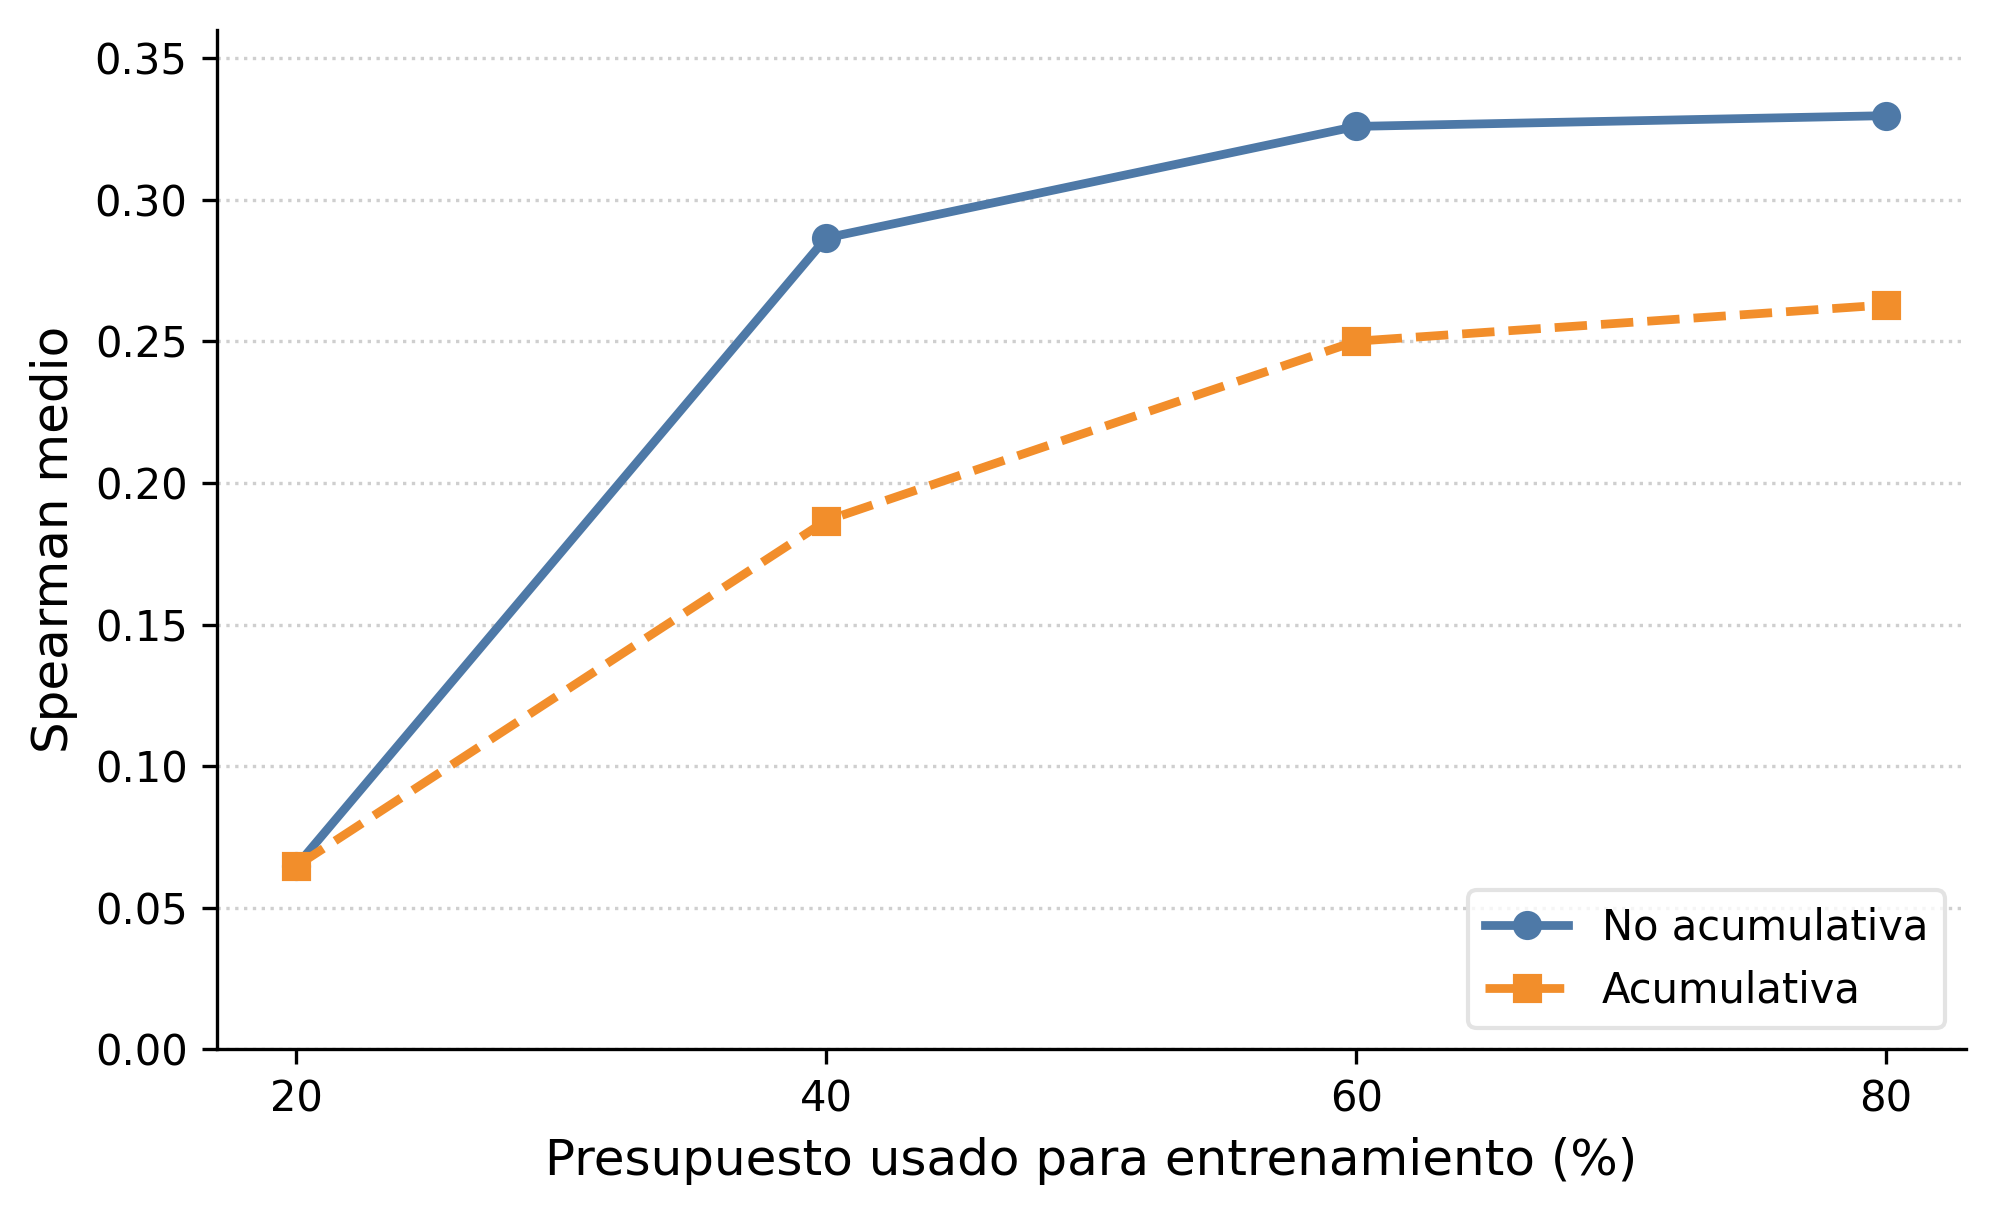
\includegraphics[width=0.8\textwidth]{figuras/surrogates_offline/evolucion_spearman_por_bloque_sin_svr.png}
%     \caption[Evolución de la correlación de Spearman media por bloque temporal para las estrategias acumulativa y no acumulativa.]{Evolución de la correlación de Spearman media por bloque temporal para las estrategias acumulativa y no acumulativa, excluyendo SVR por no completar la evaluación acumulativa.}
%     \label{fig:evolucion_spearman_bloques_offline}
% \end{figure}
\begin{figure}[H]
    \centering
    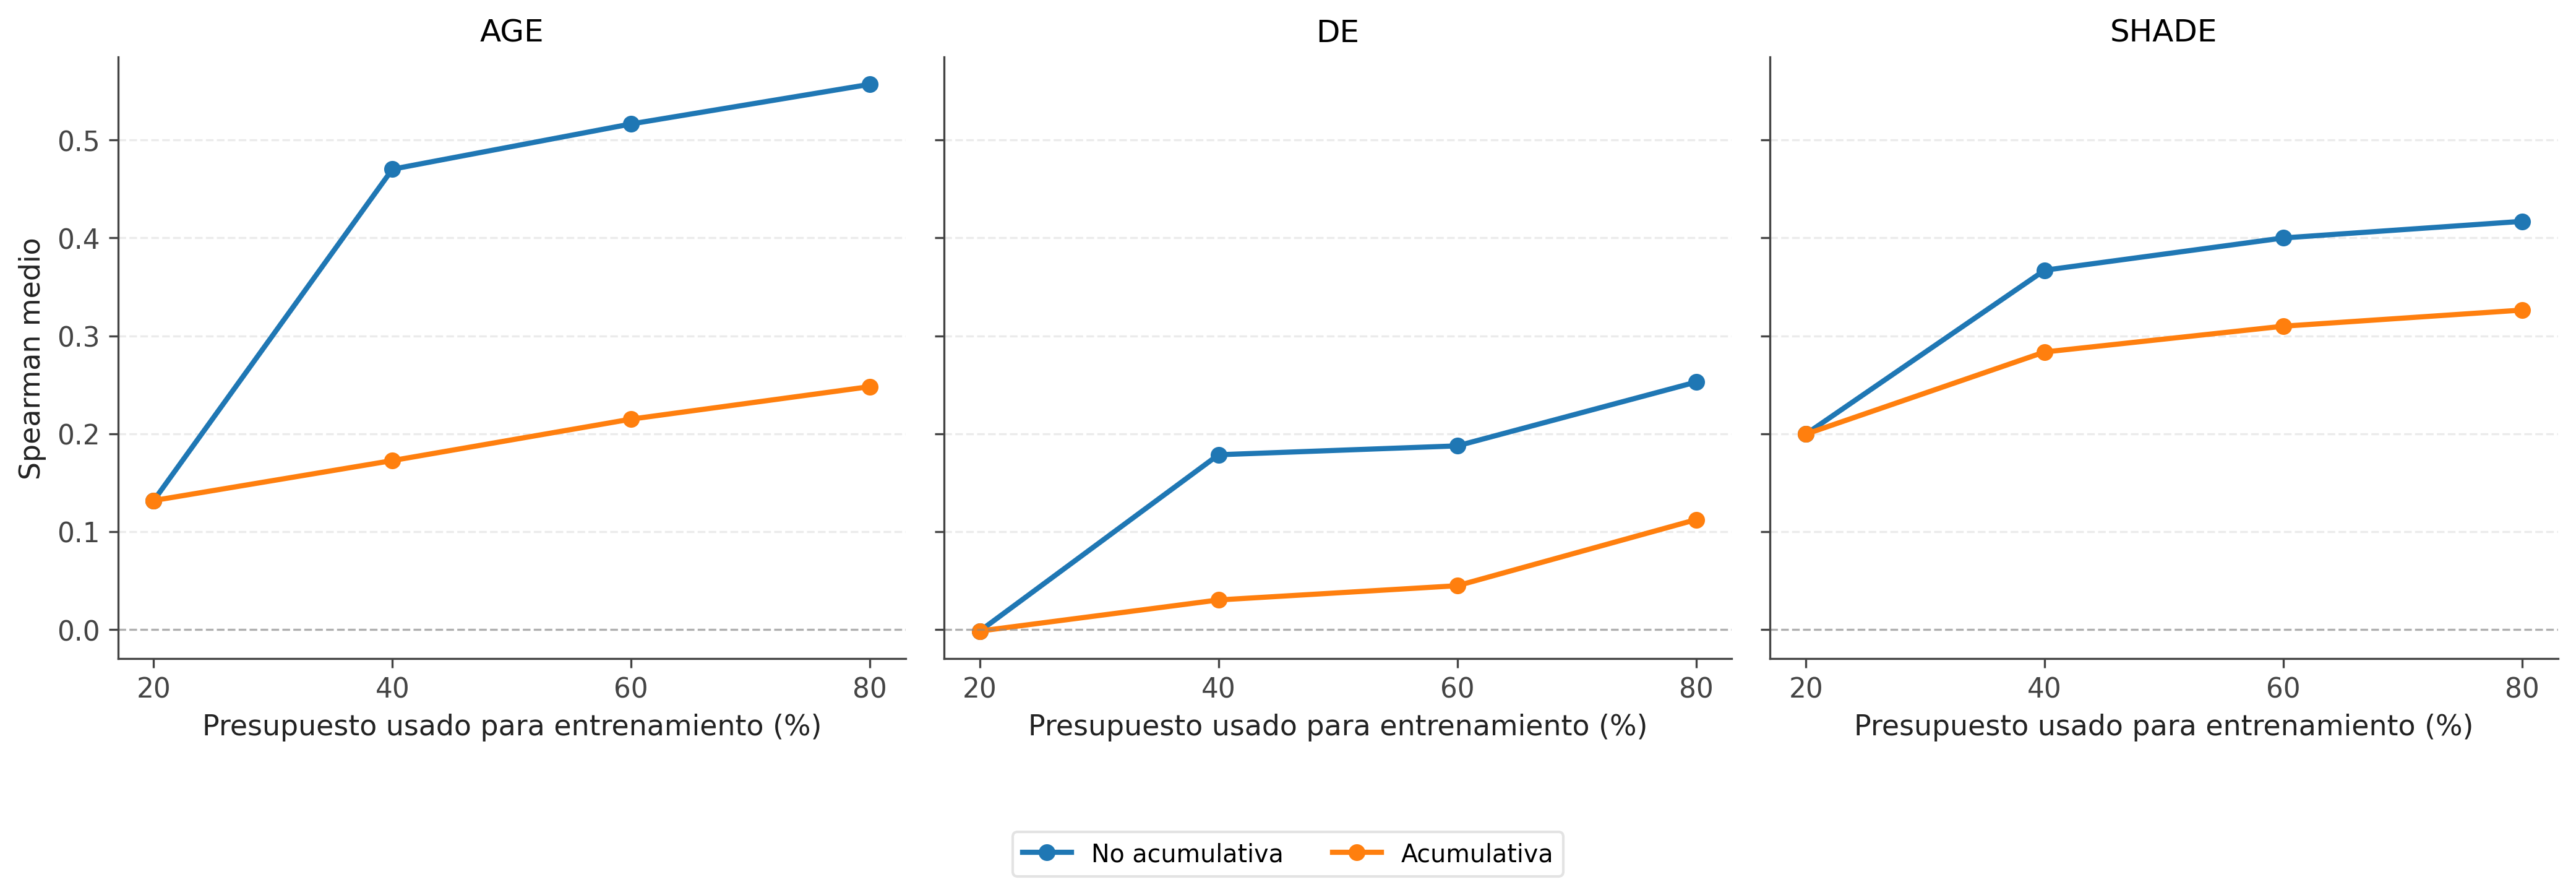
\includegraphics[width=\textwidth]{figuras/surrogates_offline/evolucion_spearman_por_bloque_por_algoritmo.png}
    \caption[Evolución de la correlación de Spearman media por bloque temporal para las estrategias acumulativa y no acumulativa.]{Evolución de la correlación de Spearman media por bloque temporal para las estrategias acumulativa y no acumulativa, desglosada por algoritmo (AGE, DE, SHADE).}
    \label{fig:evolucion_spearman_bloques_offline}
\end{figure}

La Figura~\ref{fig:evolucion_spearman_bloques_offline} confirma que la ventaja de la estrategia no acumulativa no procede de un único bloque temporal. En el primer bloque ambas estrategias parten de valores prácticamente idénticos, ya que el conjunto de entrenamiento disponible es equivalente. Sin embargo, a partir del segundo bloque la estrategia no acumulativa obtiene de forma consistente valores superiores de Spearman. Esta diferencia se mantiene hasta los bloques finales,
lo que indica que la ventaja observada en la tabla agregada no responde a un
comportamiento puntual, sino a una tendencia sostenida durante la evaluación.

Por tanto, el \textbf{enfoque no acumulativo} es la mejor opción al aislar al modelo de la influencia negativa del histórico y permitir que se concentre exclusivamente en la región temporal más reciente de la búsqueda. En consecuencia, los análisis posteriores se centran en la estrategia no acumulativa como protocolo de entrenamiento \textit{offline} de referencia.

\subsection{Competición de Modelos y Evolución por Bloques}
\label{subsec:comparacion_modelos}

Tras justificar la estrategia no acumulativa como protocolo de evaluación ideal, este apartado profundiza en el comportamiento individual de cada modelo a lo largo de la optimización, reincorporando al modelo SVR en la comparativa.

% La Figura~\ref{fig:evolucion_spearman_modelos_no_acumulativo} desglosa la evolución del coeficiente de Spearman para cada modelo bajo el esquema no acumulativo. Cada punto representa una evaluación temporal adelantada: el modelo se entrena con el último bloque disponible y se valida sobre el bloque inmediatamente posterior. Así, el punto situado en la cota del 60\% de presupuesto usado para entrenamiento corresponde al modelo ajustado con el tramo 40--60\% y validado sobre el bloque futuro 60--80\%.

La Figura~\ref{fig:evolucion_spearman_modelos_no_acumulativo} muestra cómo cambia la capacidad de ordenación de cada modelo conforme avanza la trayectoria. El primer punto corresponde al entrenamiento con el bloque inicial 0--20\% y la validación sobre el bloque 20--40\%, por lo que representa la primera situación en la que podría utilizarse un subrogado tras una fase inicial de muestreo. Los puntos posteriores permiten observar si esa capacidad de ordenación se mantiene, mejora o se degrada conforme la búsqueda avanza hacia regiones más concretas del espacio.


% \begin{figure}[H]
%     \centering
%     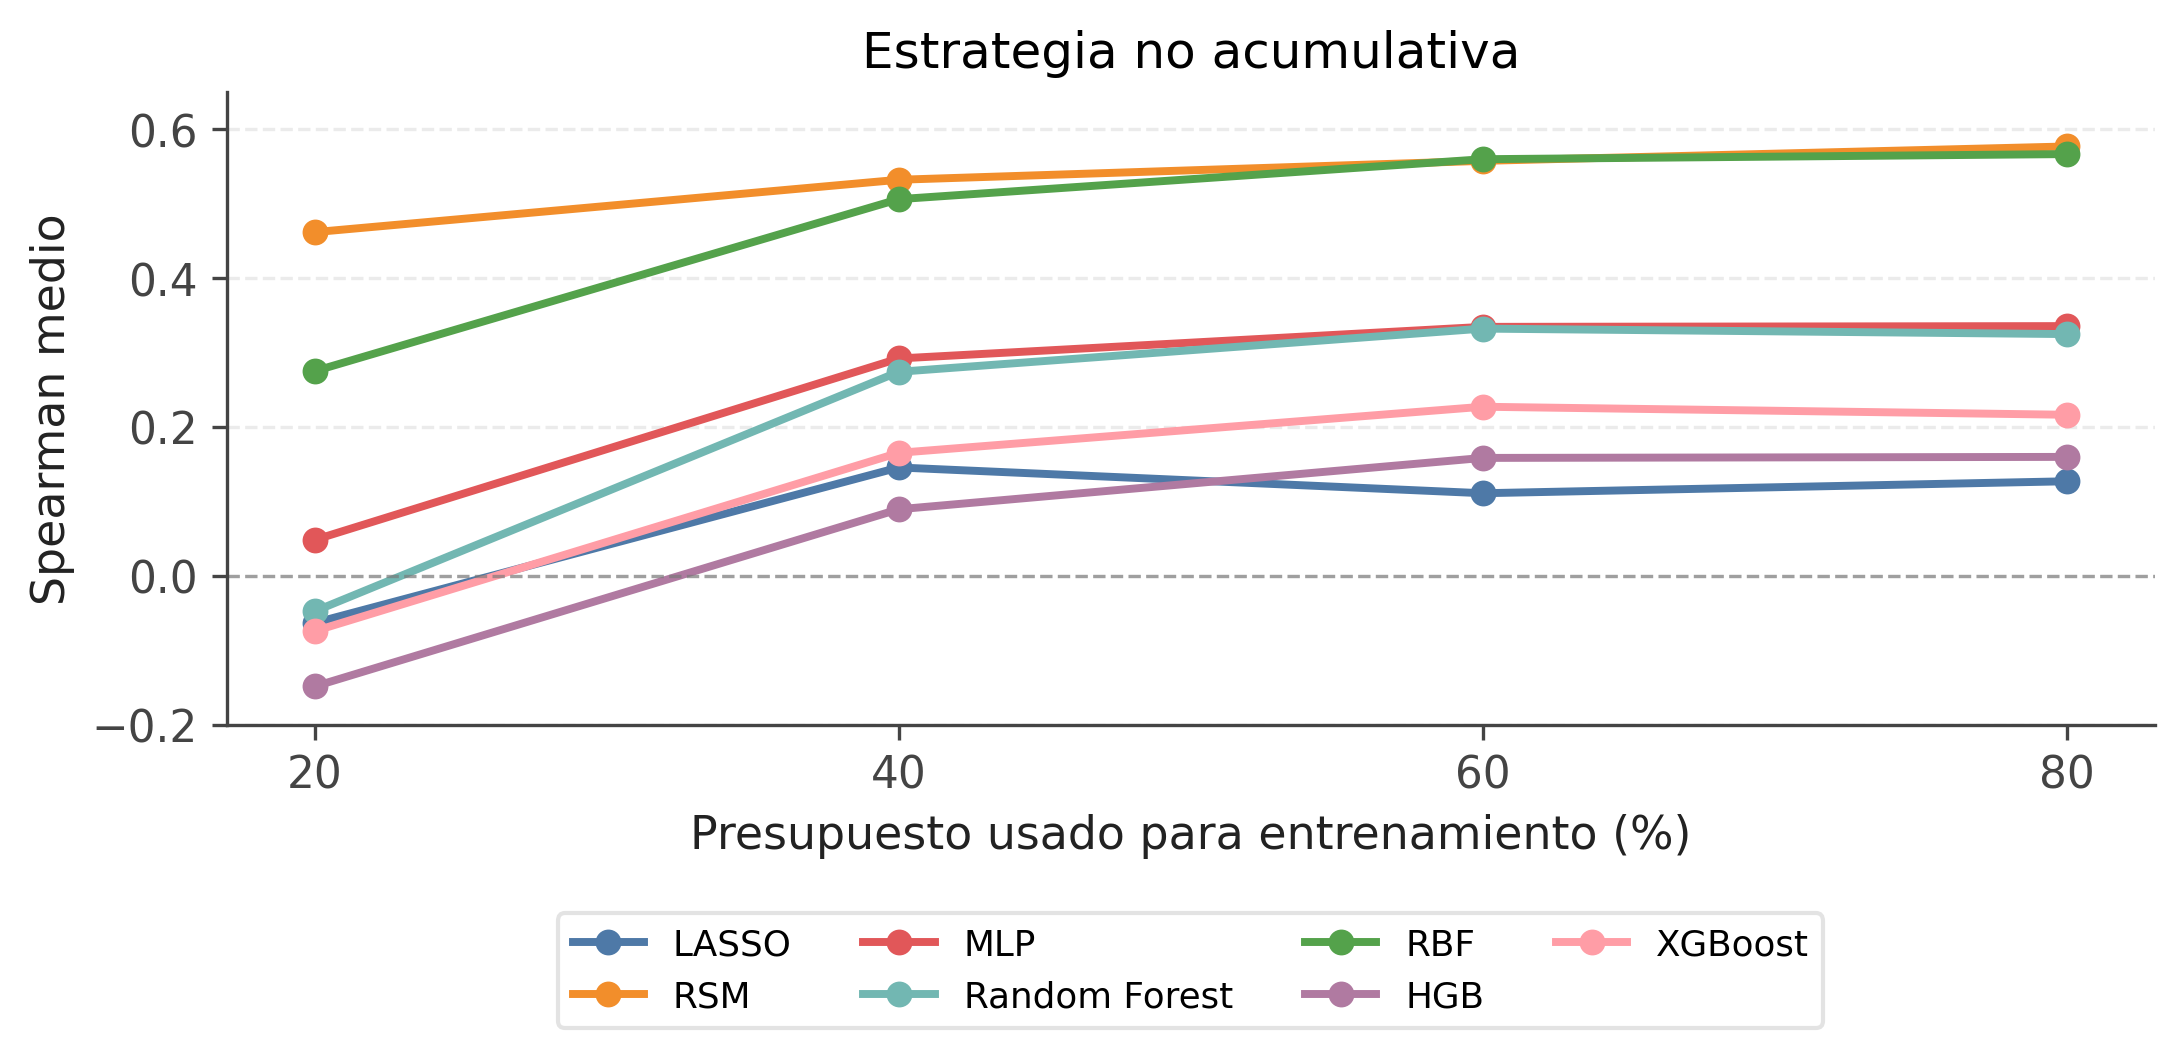
\includegraphics[width=1.0\textwidth]{figuras/surrogates_offline/evolucion_spearman_modelos_no_acumulativo.png}
%     \caption[Evolución de la correlación de Spearman media por bloques temporales bajo la estrategia no acumulativa.]{Evolución de la correlación de Spearman media por bloques temporales bajo la estrategia no acumulativa. Cada punto se obtiene entrenando con el bloque inmediatamente anterior al bloque evaluado.}
%     \label{fig:evolucion_spearman_modelos_no_acumulativo}
% \end{figure}
\begin{figure}[H]
    \centering
    \begin{subfigure}[b]{0.32\textwidth}
        \centering
        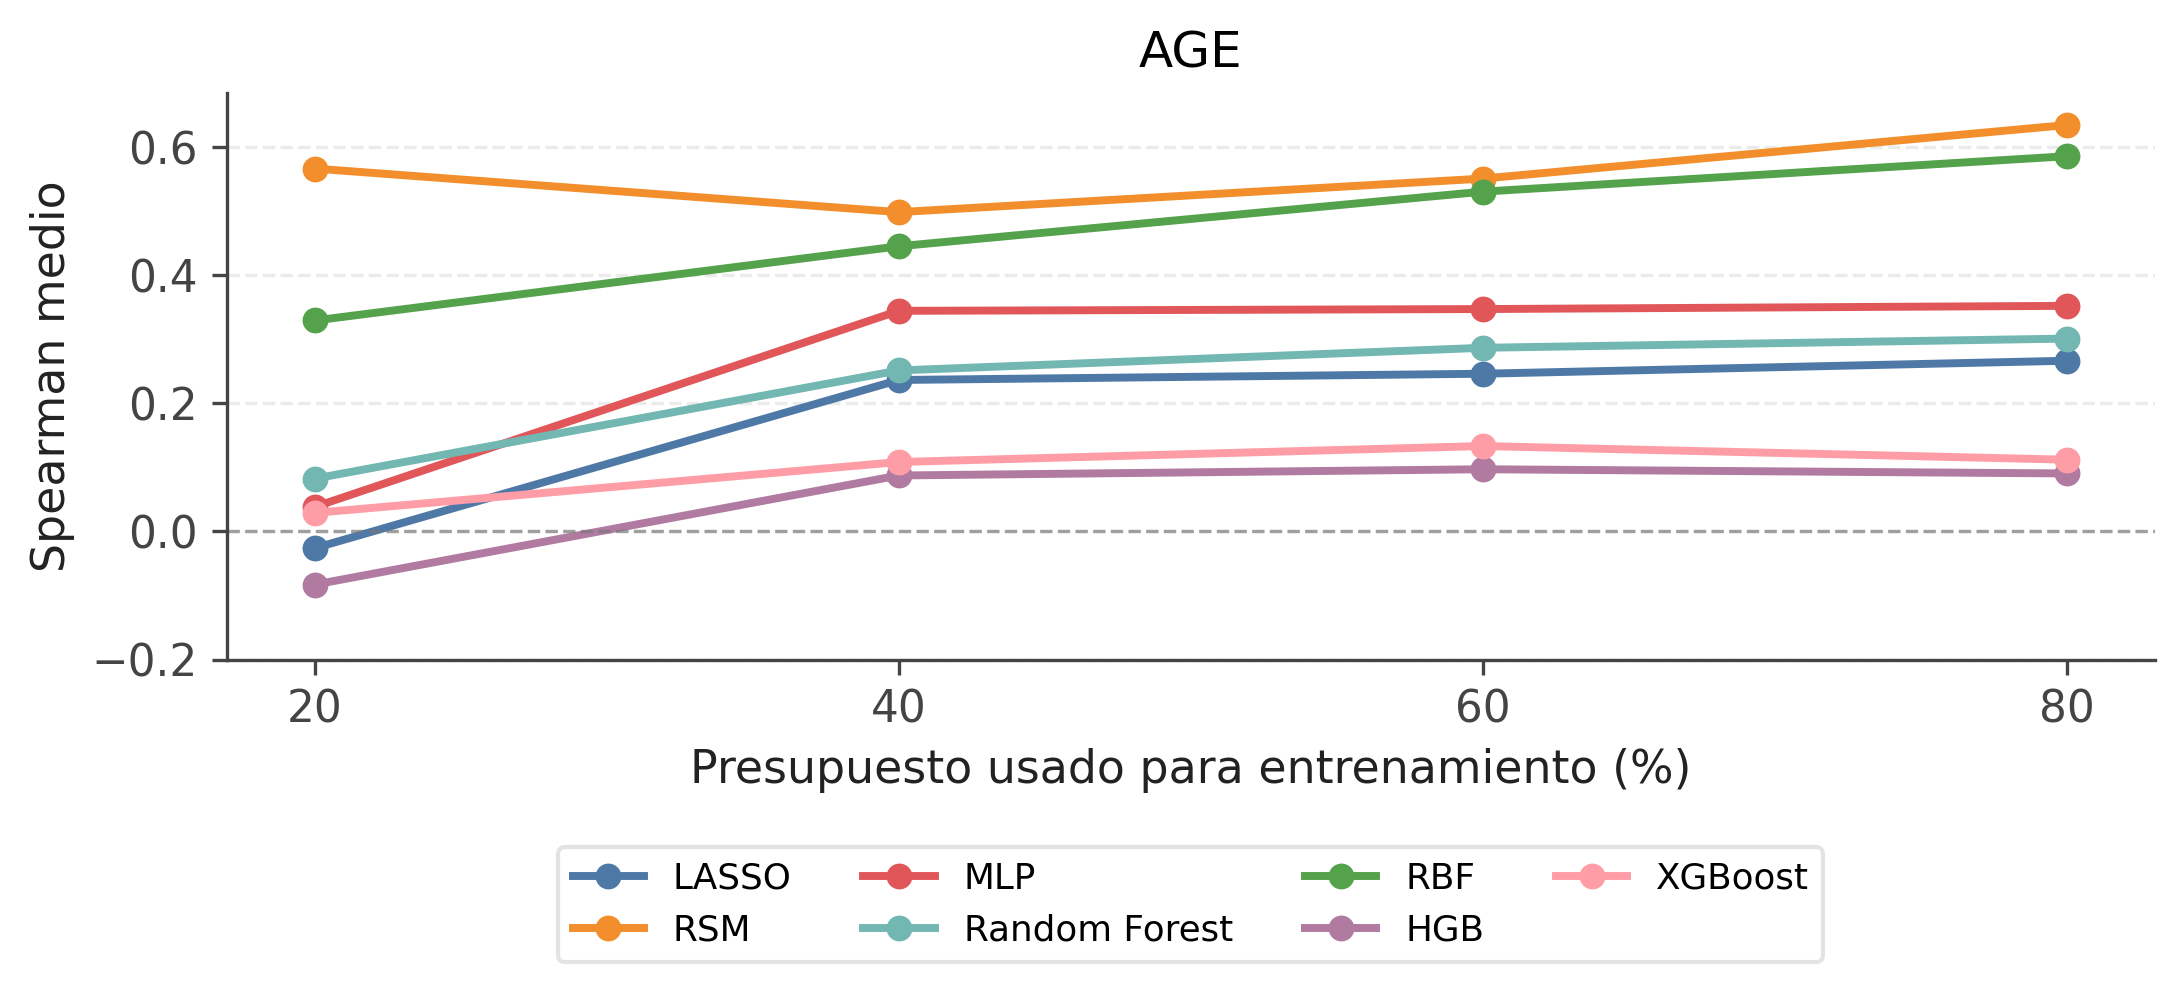
\includegraphics[width=\textwidth]{figuras/surrogates_offline/evolucion_spearman_modelos_no_acumulativo_age.png}
        \caption{AGE}
    \end{subfigure}
    \hfill
    \begin{subfigure}[b]{0.32\textwidth}
        \centering
        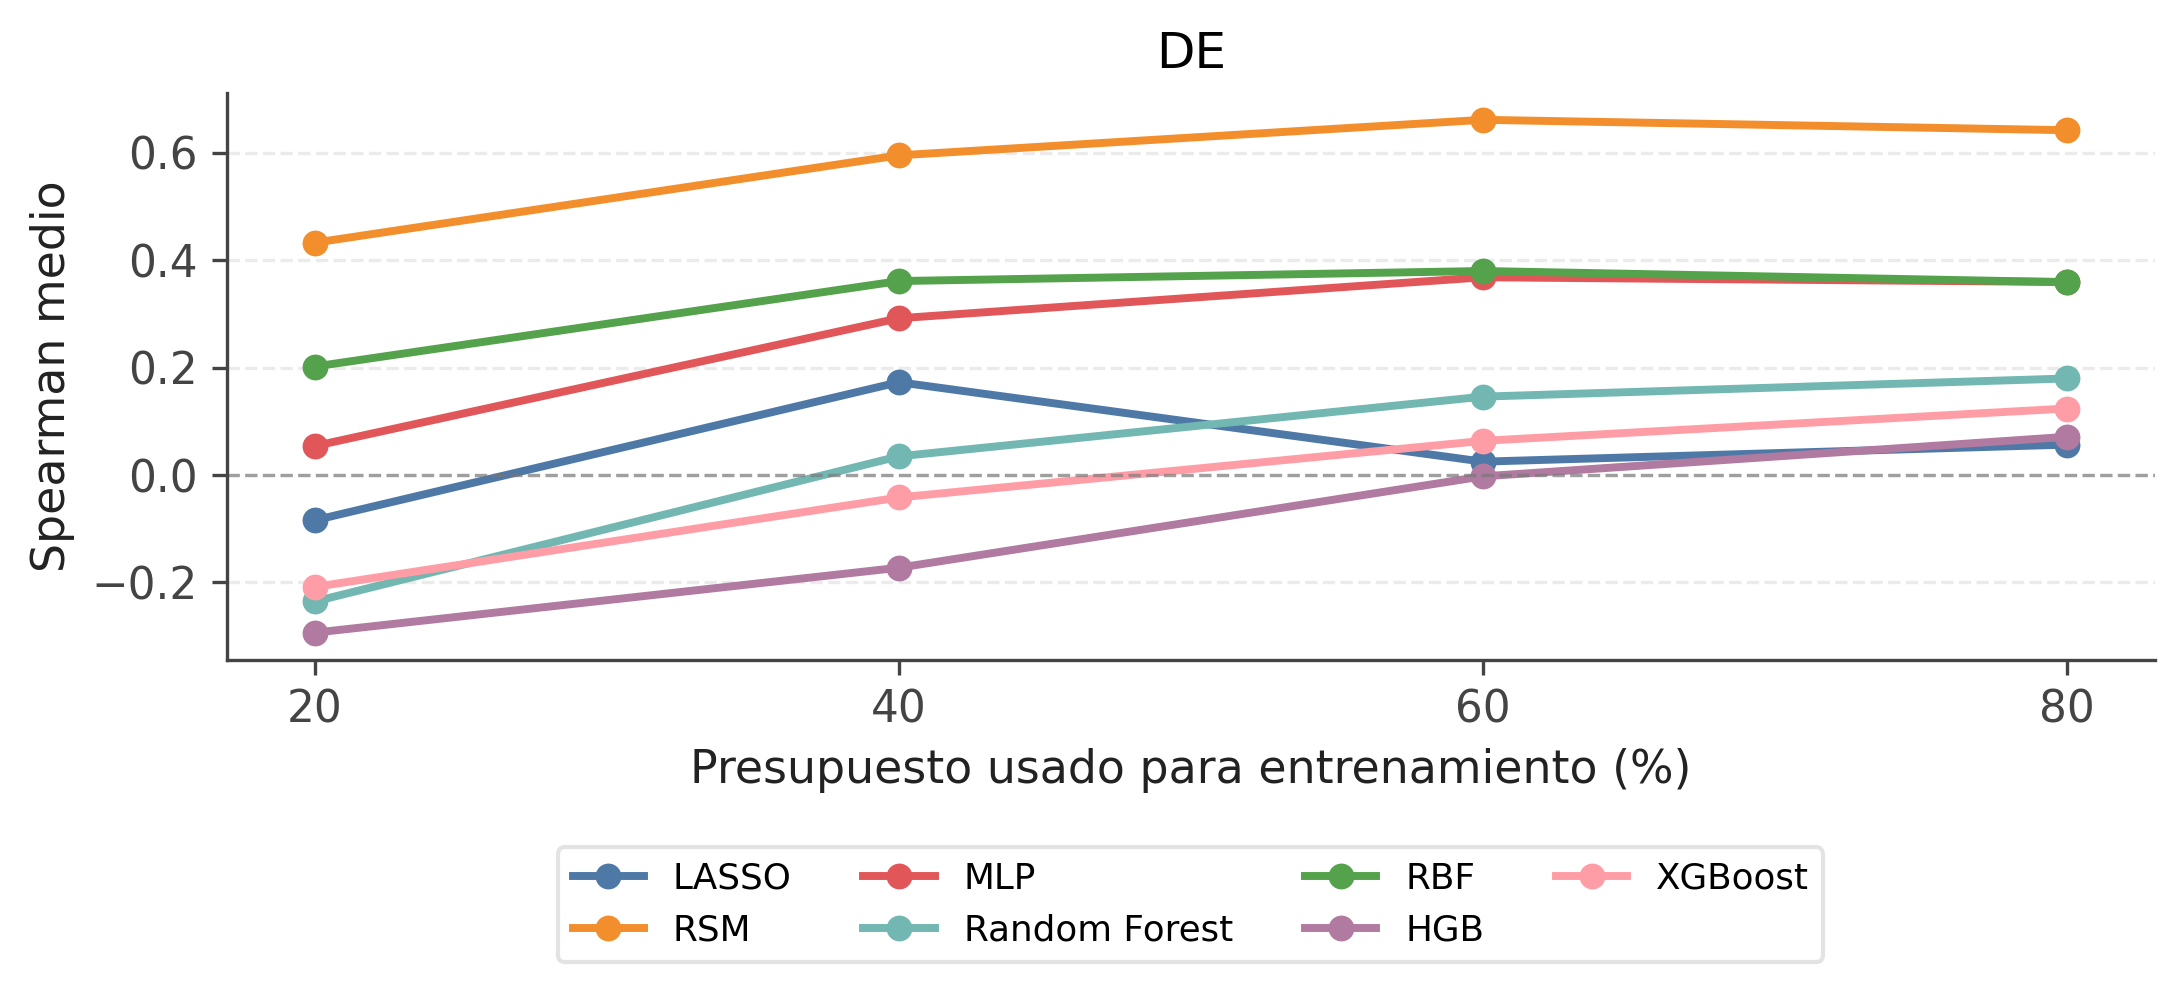
\includegraphics[width=\textwidth]{figuras/surrogates_offline/evolucion_spearman_modelos_no_acumulativo_de.png}
        \caption{DE}
    \end{subfigure}
    \hfill
    \begin{subfigure}[b]{0.32\textwidth}
        \centering
        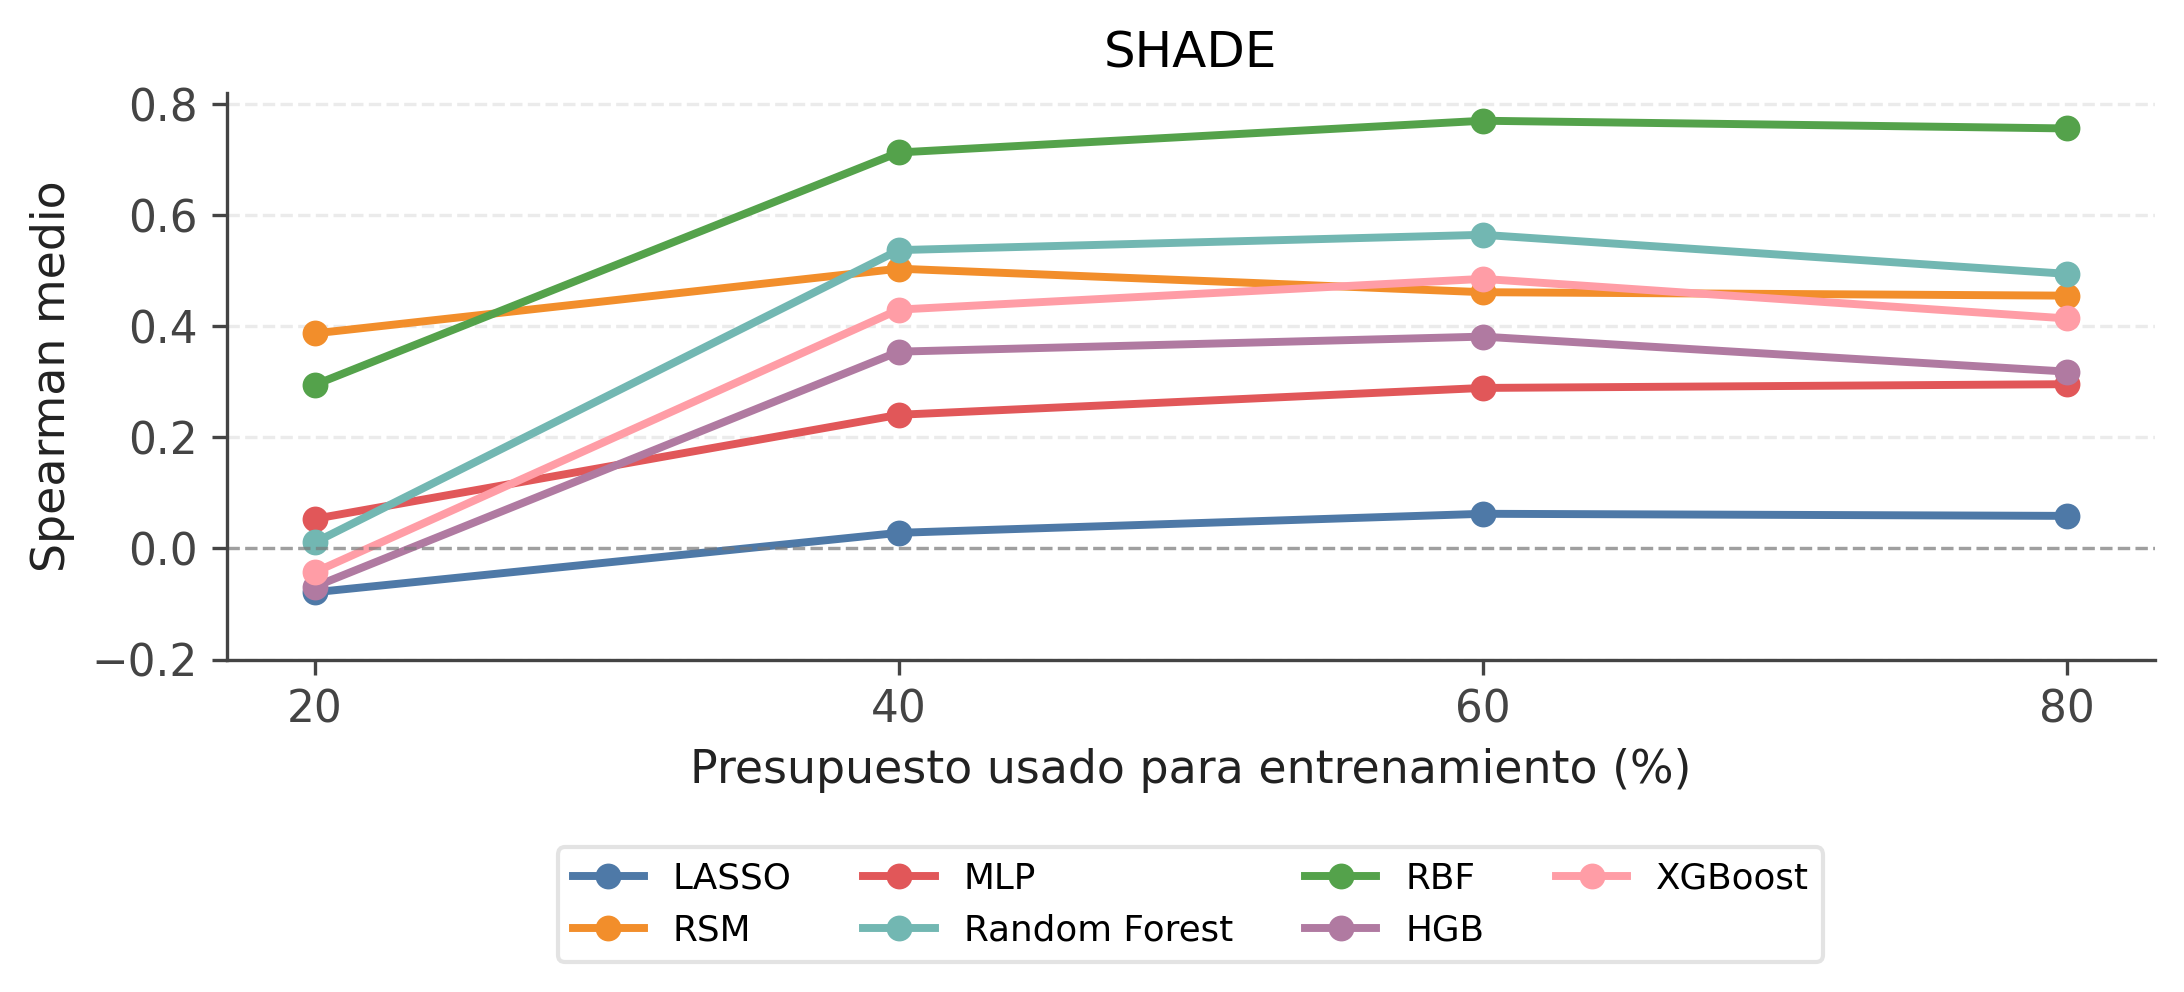
\includegraphics[width=\textwidth]{figuras/surrogates_offline/evolucion_spearman_modelos_no_acumulativo_shade.png}
        \caption{SHADE}
    \end{subfigure}
    \caption[Evolución de la correlación de Spearman media por bloques temporales bajo la estrategia no acumulativa.]{Evolución de la correlación de Spearman media por bloques temporales bajo la estrategia no acumulativa, desglosada por algoritmo. Cada punto se obtiene entrenando con el bloque inmediatamente anterior al bloque evaluado.}
    \label{fig:evolucion_spearman_modelos_no_acumulativo}
\end{figure}

Desde esta perspectiva temporal se observa una separación clara entre modelos. RSM parte con el mejor comportamiento desde el primer bloque y mantiene valores elevados durante toda la evaluación. RBF, en cambio, comienza con una correlación menor, pero mejora de forma marcada al pasar al bloque 40--60\% y, desde ese momento, se mantiene muy próximo a RSM. Esta evolución sugiere que RBF necesita trayectorias algo más estructuradas para explotar mejor la información local, mientras que RSM resulta más competitivo desde fases tempranas.

El resto de modelos también mejora respecto al primer bloque, pero su evolución se estabiliza en niveles claramente inferiores, destacando SVR, MLP o Random Forest. Por tanto, la figura no solo permite identificar qué modelos alcanzan mejores valores finales, sino también en qué momento de la trayectoria empiezan a ser útiles como aproximadores subrogados.

Las Tablas~\ref{tab:comparativa_modelos_bloques_age}, \ref{tab:comparativa_modelos_bloques_de} y \ref{tab:comparativa_modelos_bloques_shade} trasladan esa evolución a rangos concretos por bloque y algoritmo.

% \begin{table}[H]
    \centering
    \small
    \setlength{\tabcolsep}{5pt}
    \renewcommand{\arraystretch}{1.12}
    \begin{adjustbox}{max width=\textwidth}
        \begin{tabular}{l cccc ccc}
            \toprule
            \multirow{2}{*}{\textbf{Modelo}}
                             & \multicolumn{4}{c}{\textbf{Spearman por bloque de validación}}
                             & \multicolumn{3}{c}{\textbf{Media agregada}}                                                                                                                                 \\
            \cmidrule(lr){2-5} \cmidrule(lr){6-8}
                             & \textbf{20--40\%}
                             & \textbf{40--60\%}
                             & \textbf{60--80\%}
                             & \textbf{80--100\%}
                             & \textbf{nRMSE $\downarrow$}
                             & \textbf{Entren. $\downarrow$}
                             & \textbf{Pred. $\downarrow$}                                                                                                                                                 \\
            \midrule
            \rowcolor{gray!10}
            \textbf{RSM}     & \textbf{0.4620}                                                & \textbf{0.5323} & 0.5577          & \textbf{0.5771} & 266.3905         & 0.0219          & 0.0013          \\
            \rowcolor{gray!10}
            \textbf{RBF}     & 0.2752                                                         & 0.5063          & \textbf{0.5600} & 0.5668          & \textbf{12.0877} & 0.0045          & 0.4570          \\
            \addlinespace[2pt]
            \textbf{SVR}     & 0.0477                                                         & 0.3186          & 0.3472          & 0.3585          & 668.8085         & 1.3806          & 0.4042          \\
            \textbf{MLP}     & 0.0485                                                         & 0.2922          & 0.3347          & 0.3357          & 91.2443          & 1.5634          & 0.0018          \\
            \textbf{RF}      & -0.0475                                                        & 0.2743          & 0.3323          & 0.3250          & 17.0255          & 1.8417          & 0.0414          \\
            \textbf{XGBoost} & -0.0742                                                        & 0.1654          & 0.2273          & 0.2165          & 19.2891          & 0.5254          & 0.0032          \\
            \textbf{HGB}     & -0.1485                                                        & 0.0896          & 0.1585          & 0.1599          & 47.2223          & 0.6218          & 0.0150          \\
            \textbf{LASSO}   & -0.0631                                                        & 0.1457          & 0.1111          & 0.1272          & 388.9506         & \textbf{0.0009} & \textbf{0.0001} \\
            \bottomrule
        \end{tabular}
    \end{adjustbox}
    \caption{Comparativa de modelos bajo la estrategia no acumulativa.}
    \label{tab:comparativa_modelos_bloques_informativos}
\end{table}
% \begin{table}[H]
    \centering
    \small
    \begin{adjustbox}{max width=\textwidth}
\begin{tabular}{l r r r r r r}
\toprule
\textbf{Modelo} & \textbf{Rank AGE} & \textbf{Rank DE} & \textbf{Rank SHADE} & \textbf{Rank medio} & \textbf{Entren. (s)} & \textbf{Pred. (s)} \\
\midrule
RBF & \textbf{1.71} & \textbf{1.58} & \textbf{1.29} & \textbf{1.53} & 0.0040 & 0.3041 \\
XGBoost & 3.25 & 3.67 & 3.50 & 3.47 & 0.3902 & 0.0022 \\
RF & 4.21 & 3.88 & 2.54 & 3.54 & 1.1527 & 0.0347 \\
RSM & 2.33 & 4.50 & 5.67 & 4.17 & 0.0150 & 0.0009 \\
HGB & 4.71 & 3.96 & 4.25 & 4.31 & 0.3207 & 0.0083 \\
MLP & 5.33 & 4.50 & 4.50 & 4.78 & 1.2387 & 0.0011 \\
LASSO & 6.46 & 4.54 & 5.12 & 5.38 & \textbf{0.0006} & \textbf{0.0000} \\
\bottomrule
\end{tabular}
    \end{adjustbox}
    \caption{Competición de modelos bajo la estrategia no acumulativa. Rank~AGE/DE/SHADE: posición media (1\,=\,mejor Spearman) sobre funciones~$\times$~bloques de validación para cada algoritmo. Tiempos agregados sobre algoritmos, funciones y bloques.}
    \label{tab:comparativa_modelos_offline_v2}
\end{table}
\begin{table}[H]
    \centering
    \small
    \setlength{\tabcolsep}{4pt}
    \begin{adjustbox}{max width=\textwidth}
        \begin{tabular}{lrrrr|rr}
            \toprule
            \multicolumn{1}{l}{} & \multicolumn{4}{c}{\textbf{Rank medio por bloque}} & \multicolumn{2}{c}{\textbf{Tiempos medios}}                                                                               \\
            \cmidrule(lr){2-5} \cmidrule(lr){6-7}
            \textbf{Modelo}      & \textbf{20\%}                                      & \textbf{40\%}                               & \textbf{60\%} & \textbf{80\%} & \textbf{Entren.\ (s)} & \textbf{Pred.\ (s)} \\
            \midrule
            RBF                  & \textbf{1.67}                                      & 2.17                                        & \textbf{1.67} & \textbf{1.33} & 0.0041                & 0.4302              \\
            RSM                  & 3.17                                               & \textbf{1.83}                               & 1.83          & 2.50          & 0.0151                & 0.0009              \\
            XGBoost              & 4.50                                               & 3.17                                        & 2.83          & 2.50          & 0.4229                & 0.0024              \\
            RF                   & 3.00                                               & 4.67                                        & 4.50          & 4.67          & 0.8222                & 0.0377              \\
            HGB                  & 6.17                                               & 4.50                                        & 4.17          & 4.00          & 0.3957                & 0.0103              \\
            MLP                  & 4.00                                               & 5.33                                        & 6.00          & 6.00          & 0.5730                & 0.0011              \\
            LASSO                & 5.50                                               & 6.33                                        & 7.00          & 7.00          & \textbf{0.0006}       & \textbf{0.0000}     \\
            \bottomrule
        \end{tabular}
    \end{adjustbox}
    \caption{Competición de modelos para AGE bajo la estrategia no acumulativa, desglosada por bloque temporal. Rank medio calculado sobre las funciones de prueba para cada bloque de validación (1\,=\,mejor Spearman). Tiempos agregados sobre funciones y bloques.}
    \label{tab:comparativa_modelos_bloques_age}
\end{table}

\begin{table}[H]
    \centering
    \small
    \setlength{\tabcolsep}{4pt}
    \begin{adjustbox}{max width=\textwidth}
        \begin{tabular}{lrrrr|rr}
            \toprule
            \multicolumn{1}{l}{} & \multicolumn{4}{c}{\textbf{Rank medio por bloque}} & \multicolumn{2}{c}{\textbf{Tiempos medios}} \\
            \cmidrule(lr){2-5} \cmidrule(lr){6-7}
            \textbf{Modelo} & \textbf{20\%} & \textbf{40\%} & \textbf{60\%} & \textbf{80\%} & \textbf{Entren.\ (s)} & \textbf{Pred.\ (s)} \\
            \midrule
            RBF & \textbf{2.00} & \textbf{1.67} & \textbf{1.33} & \textbf{1.33} & 0.0039 & 0.2304 \\
            XGBoost & 5.17 & 3.67 & 4.00 & 3.50 & 0.3616 & 0.0020 \\
            HGB & 5.83 & 4.33 & 3.83 & 2.83 & 0.3117 & 0.0079 \\
            RF & 5.33 & 4.17 & 3.67 & 4.00 & 1.3868 & 0.0317 \\
            MLP & 2.67 & 4.50 & 5.00 & 5.83 & 1.5273 & 0.0011 \\
            RSM & 3.00 & 4.83 & 5.00 & 5.17 & 0.0150 & 0.0009 \\
            LASSO & 4.00 & 4.83 & 5.17 & 5.33 & \textbf{0.0006} & \textbf{0.0000} \\
            \bottomrule
        \end{tabular}
    \end{adjustbox}
    \caption{Competición de modelos para DE bajo la estrategia no acumulativa, desglosada por bloque temporal. Rank medio calculado sobre las funciones de prueba para cada bloque de validación (1\,=\,mejor Spearman). Tiempos agregados sobre funciones y bloques.}
    \label{tab:comparativa_modelos_bloques_de}
\end{table}

\begin{table}[H]
    \centering
    \small
    \setlength{\tabcolsep}{4pt}
    \begin{adjustbox}{max width=\textwidth}
        \begin{tabular}{lrrrr|rr}
            \toprule
            \multicolumn{1}{l}{} & \multicolumn{4}{c}{\textbf{Rank medio por bloque}} & \multicolumn{2}{c}{\textbf{Tiempos medios}} \\
            \cmidrule(lr){2-5} \cmidrule(lr){6-7}
            \textbf{Modelo} & \textbf{20\%} & \textbf{40\%} & \textbf{60\%} & \textbf{80\%} & \textbf{Entren.\ (s)} & \textbf{Pred.\ (s)} \\
            \midrule
            RBF & \textbf{1.83} & \textbf{1.17} & \textbf{1.17} & \textbf{1.00} & 0.0040 & 0.2518 \\
            RF & 2.83 & 2.75 & 2.83 & 3.17 & 1.2491 & 0.0346 \\
            XGBoost & 4.00 & 3.75 & 3.83 & 3.83 & 0.3860 & 0.0022 \\
            HGB & 5.00 & 4.42 & 4.17 & 4.00 & 0.2548 & 0.0068 \\
            MLP & 4.50 & 4.67 & 4.50 & 4.33 & 1.6158 & 0.0011 \\
            LASSO & 4.83 & 5.42 & 5.67 & 5.67 & \textbf{0.0006} & \textbf{0.0000} \\
            RSM & 5.00 & 5.83 & 5.83 & 6.00 & 0.0150 & 0.0009 \\
            \bottomrule
        \end{tabular}
    \end{adjustbox}
    \caption{Competición de modelos para SHADE bajo la estrategia no acumulativa, desglosada por bloque temporal. Rank medio calculado sobre las funciones de prueba para cada bloque de validación (1\,=\,mejor Spearman). Tiempos agregados sobre funciones y bloques.}
    \label{tab:comparativa_modelos_bloques_shade}
\end{table}


% Al considerar estas métricas adicionales, la comparación entre RSM y RBF queda más equilibrada, aunque siguen siendo las alternativas más competitivas del conjunto de modelos evaluados. RSM mantiene una mayor capacidad de ordenación en la mayoría de bloques y presenta un tiempo de predicción muy reducido, pero su error normalizado es considerablemente más elevado. RBF, por su parte, obtiene un error menor y un tiempo de entrenamiento bajo, aunque su coste de predicción es superior. Por tanto, ninguno de los dos modelos domina al otro en todas las métricas, lo que justifica mantener ambos como candidatos para las siguientes fases experimentales.

% La viabilidad del resto de regresores se ve limitada por no satisfacer simultáneamente los criterios descritos en el capítulo anterior. Modelos como SVR ($1.38$~s), MLP ($1.56$~s) y Random Forest ($1.84$~s) mejoran conforme avanza la búsqueda, pero no alcanzan los valores de Spearman de RSM y RBF y requieren tiempos de entrenamiento muy altos. En cambio, LASSO y los modelos de \textit{boosting} presentan costes más contenidos, pero su capacidad para preservar el orden relativo entre soluciones resulta insuficiente.

En los tres algoritmos, RBF encabeza la clasificación de forma consistente y consolida su ventaja en los bloques finales, confirmando la tendencia que la figura ya anticipaba visualmente. El resto de modelos queda descartado por no cumplir simultáneamente los criterios de fidelidad ordinal y coste computacional: Random Forest, MLP y SVR mejoran conforme avanza la búsqueda pero presentan tiempos de entrenamiento demasiado elevados para la integración \textit{online}, mientras que LASSO y los modelos de \textit{boosting} resultan más eficientes pero no alcanzan una capacidad de ordenación suficiente. RSM muestra un comportamiento dependiente del algoritmo: es competitivo para AGE durante toda la evaluación, pero su rango empeora progresivamente en DE y SHADE, lo que evidencia que su ventaja en fases tempranas no se sostiene a largo plazo y que el análisis agregado habría ocultado esta diferencia.

En consecuencia, tras validar empíricamente la ventaja de la estrategia no
acumulativa, la integración \textit{online} se planteará siguiendo una lógica de \textbf{ventana deslizante}, utilizando la información más reciente de la trayectoria para entrenar el subrogado. Los valores obtenidos en el bloque 20--40\% muestran que el tramo inicial de calentamiento \(0\)--\(20\%\) ya permite construir un primer modelo con cierta capacidad de ordenación, especialmente en el caso de \textbf{RSM}. Sin embargo, la comparación conjunta de Spearman, error normalizado y coste computacional no permite descartar aún a \textbf{RBF}, que muestra un comportamiento más equilibrado en varias de las métricas agregadas.

Por tanto, la fase de cribado reduce la comparativa a dos candidatos
principales, \textbf{RSM} y \textbf{RBF}. El siguiente paso consiste en ajustar sus hiperparámetros para comprobar si alguno de ellos ofrece una ventaja más clara antes de abordar la integración \textit{online}.

\subsection{Ajuste Fino de Hiperparámetros}

El ajuste fino se plantea como una comparación controlada entre las
configuraciones candidatas de \textbf{RBF} y \textbf{RSM}.

Siguiendo el protocolo descrito en la Sección~\ref{sec:protocolo_ajuste_hiperparametros}, las configuraciones candidatas se comparan mediante \textbf{validación interna} dentro del propio bloque de entrenamiento y se evalúan posteriormente sobre el bloque temporal inmediatamente posterior.

Dado que el coste de ambos modelos no es equivalente, el número de semillas
empleado en el ajuste no se fija de forma uniforme. Como muestra la
Tabla~\ref{tab:comparativa_modelos_bloques_informativos}, \textbf{RSM} presenta un tiempo medio de predicción muy reducido, por lo que su espacio de búsqueda se evalúa utilizando las \(51\) semillas disponibles. En cambio, \textbf{RBF} mantiene un tiempo de entrenamiento bajo, pero su tiempo medio de predicción es bastante superior. Por este motivo, su ajuste se realiza sobre un subconjunto fijo de \(10\) semillas, evitando que la exploración de hiperparámetros quede dominada por el coste de predicción.

Los valores concretos del espacio de búsqueda para ambos modelos se recogen en la Tabla~\ref{tab:grid_hiperparametros_rbf_rsm}, evaluando 36 configuraciones para RBF y 3 para RSM en cada validación interna.

\begin{table}[htbp]
    \centering
    \small
    \setlength{\tabcolsep}{4pt}
    \begin{tabular}{lll}
        \toprule
        \textbf{Modelo} & \textbf{Hiperparámetro} & \textbf{Valores}       \\
        \midrule
        RBF             & kernel                  & multiquadric, gaussian \\
        RBF             & epsilon                 & 0.1, 1.0, 10.0         \\
        RBF             & smoothing               & $10^{-3}$, $10^{-2}$   \\
        RBF             & vecinos                 & 25, 50, 100            \\
        RBF             & degree                  & -1                     \\
        RSM             & degree                  & 1, 2, 3                \\
        \bottomrule
    \end{tabular}
    \caption{Espacio de búsqueda utilizado en el ajuste fino de hiperparámetros.}
    \label{tab:grid_hiperparametros_rbf_rsm}
\end{table}


La Tabla~\ref{tab:ajuste_interno_rsm} y la Tabla~\ref{tab:ajuste_interno_rbf} resumen las configuraciones más relevantes. En el caso de \textbf{RSM} se muestran las \textbf{tres configuraciones} evaluadas mientras que, para \textbf{RBF}, debido a un espacio de búsqueda mayor, se recogen las \textbf{cinco mejores configuraciones} según Spearman. Esta selección permite observar si la configuración con mayor correlación ordinal resulta también adecuada al considerar el error normalizado y el coste computacional.

\begin{table}[H]
    \centering
    \small
    \begin{tabular}{l|ccccc}
        \toprule
        \textbf{Grado} & \textbf{Spearman} & \textbf{nRMSE}   & \textbf{nMAE}    & \textbf{Entren. (s)} & \textbf{Pred. (s)} \\
        \midrule
        1              & 0.1010            & 102437.7634      & 102411.6769      & \textbf{0.0041}      & \textbf{0.0003}    \\
        2              & 0.5171            & \textbf{37.6751} & \textbf{15.8988} & 0.0210               & 0.0013             \\
        3              & \textbf{0.5397}   & 12806.1889       & 3726.0165        & 0.1217               & 0.0036             \\
        \bottomrule
    \end{tabular}
    \caption{Resultados de validación interna para las configuraciones evaluadas de RSM.}
    \label{tab:ajuste_interno_rsm}
\end{table}

\begin{table}[H]
    \centering
    \small
    \setlength{\tabcolsep}{4pt}
    \begin{adjustbox}{max width=\textwidth}
        \begin{tabular}{ll|rrrrr}
            \toprule
            \textbf{Smoothing} & \textbf{Vecinos} & \textbf{Spearman} & \textbf{nRMSE}   & \textbf{nMAE}   & \textbf{Entren. (s)} & \textbf{Pred. (s)} \\
            \midrule
            \(10^{-3}\)        & 100              & \textbf{0.5060}   & \textbf{31.0542} & \textbf{5.6335} & 0.0030               & 0.4034             \\
            \(10^{-2}\)        & 25               & 0.5032            & 189.0826         & 165.9680        & 0.0030               & \textbf{0.1654}    \\
            \(10^{-3}\)        & 50               & 0.5024            & 33.3857          & 9.6081          & 0.0030               & 0.2395             \\
            \(10^{-3}\)        & 25               & 0.5002            & 39.9942          & 17.7802         & 0.0030               & 0.1660             \\
            \(10^{-2}\)        & 50               & 0.4971            & 108.0347         & 83.7609         & 0.0030               & 0.2390             \\
            \bottomrule
        \end{tabular}
    \end{adjustbox}
    \caption[Cinco mejores configuraciones de RBF según Spearman interno.]{Cinco mejores configuraciones de RBF según Spearman interno. En todas ellas se utiliza \(\text{kernel}=\textit{multiquadric}\), \(\epsilon=1.0\) y \(\text{degree}=-1\).}
    \label{tab:ajuste_interno_rbf}
\end{table}

Los resultados muestran que la configuración con mayor Spearman obtenido en la validación interna no siempre representa la opción más equilibrada para una integración \textit{online}. En \textbf{RBF}, la configuración con \(100\) vecinos obtiene el \textbf{mejor Spearman} y también los \textbf{mejores valores de error} entre las configuraciones mostradas. Sin embargo, la variante con \(50\) vecinos y el mismo núcleo \textit{multiquadric} mantiene un comportamiento prácticamente equivalente y un \textbf{tiempo de predicción claramente inferior}.

En \textbf{RSM}, la configuración con grado \(3\) obtiene el \textbf{mayor Spearman}, pero presenta errores normalizados demasiado elevados, al igual que con grado \(1\), y un mayor tiempo de entrenamiento. Por ello, aunque reduce levemente la capacidad de ordenación, el grado \(2\) muestra un compromiso más sólido entre error, Spearman y coste computacional.


Por tanto, aplicando el criterio definido en la Subsección~\ref{subsec:criterio_comparacion_modelos}, no se selecciona la configuración con mayor Spearman, sino aquella que ofrece un compromiso más adecuado entre capacidad de ordenación y coste computacional, utilizando el error normalizado como métricas secundarias:

\begin{table}[H]
    \centering
    \small
    \begin{adjustbox}{max width=\textwidth}
        \begin{tabular}{ll}
            \toprule
            \textbf{Modelo} & \textbf{Configuración seleccionada}                                                                             \\
            \midrule
            RSM             & degree \(=2\)                                                                                                   \\
            RBF             & kernel \textit{multiquadric}, \(\epsilon=1.0\), \textit{smoothing} \(=10^{-3}\), \(50\) vecinos, degree \(=-1\) \\
            \bottomrule
        \end{tabular}
    \end{adjustbox}
    \caption{Configuraciones seleccionadas tras el ajuste fino de hiperparámetros.}
    \label{tab:configuraciones_finales_ajuste_fino}
\end{table}

Para cerrar el ajuste de hiperparámetros, la Tabla~\ref{tab:comparativa_defecto_ajustado} compara las configuraciones seleccionadas frente a las iniciales empleadas en el cribado de modelos bajo las mismas condiciones.

Como la configuración final para RSM se corresponde con la misma definida en la Tabla \ref{tab:grid_hiperparametros_rbf_rsm}, se muestra únicamente RBF:

\begin{table}[H]
    \centering
    \small
    \setlength{\tabcolsep}{4pt}
    \begin{adjustbox}{max width=\textwidth}
        \begin{tabular}{llrrrrr}
            \toprule
            \textbf{Modelo} & \textbf{Configuración} & \textbf{Spearman} & \textbf{nRMSE}   & \textbf{nMAE}   & \textbf{Entren. (s)} & \textbf{Pred. (s)} \\
            \midrule
            RBF             & Inicial                & 0.4771            & \textbf{22.1669} & \textbf{2.9463} & 0.0045               & 0.4570             \\
            \midrule
            RBF             & Ajustada               & \textbf{0.5288}   & 29.8760          & 6.0312          & \textbf{0.0035}      & \textbf{0.3415}    \\
            \bottomrule
        \end{tabular}
    \end{adjustbox}
    \caption[Comparación agregada entre la configuración inicial y la seleccionada de RBF tras el ajuste de hiperparámetros] {Comparación agregada entre la configuración inicial y la seleccionada de RBF tras el ajuste de hiperparámetros sobre las funciones utilizadas en el cribado \textit{offline}.}
    \label{tab:comparativa_defecto_ajustado}
\end{table}

La versión ajustada confirma la mejora de las propiedades relevantes para la integración \textit{online}, a pesar de un incremento de los errores normalizados. El siguiente paso consiste en comprobar si este comportamiento es generalizado o sesgado al subconjunto de funciones evaluadoz.

\section{Resultados de los modelos ajustados}

Con las configuraciones fijadas, se comprueba si el comportamiento observado se mantiene al ampliar el conjunto de evaluación.

La Tabla~\ref{tab:comparativa_configuraciones_ajustadas} recoge los resultados agregados obtenidos por RSM y RBF tras aplicar las configuraciones seleccionadas sobre la suite completa CEC2017 y las \(51\) semillas empleadas en la generación de trayectorias.

\begin{table}[H]
    \centering
    \small
    \setlength{\tabcolsep}{4pt}
    \begin{adjustbox}{max width=\textwidth}
        \begin{tabular}{lccccc}
            \toprule
            \textbf{Modelo} & \textbf{Spearman} & \textbf{nRMSE}                  & \textbf{nMAE}                   & \textbf{Entren. (s)} & \textbf{Pred. (s)} \\
            \midrule
            RSM             & 0.3588            & \(5.9898 \times 10^{11}\)       & \(5.0876 \times 10^{11}\)       & 0.0242               & \textbf{0.0014}    \\
            RBF             & \textbf{0.5074}   & \(\mathbf{1.2389 \times 10^9}\) & \(\mathbf{9.5968 \times 10^8}\) & \textbf{0.0057}      & 0.7076             \\
            \bottomrule
        \end{tabular}
    \end{adjustbox}
    \caption{Comparación agregada de las configuraciones seleccionadas para RSM y RBF sobre todas las funciones de CEC2017 y las 51 semillas.}
    \label{tab:comparativa_configuraciones_ajustadas}
\end{table}

Los resultados confirman que \textbf{RBF supera a RSM} en correlación de Spearman, que constituye el criterio principal de comparación definido en el Capítulo~\ref{chap:metodologia_experimental}. Para comprobar si esta diferencia agregada se mantiene de forma homogénea o depende de familias concretas del benchmark, la Figura~\ref{fig:heatmap_spearman_final_cec2017} desagrega el coeficiente de Spearman por función y modelo.

\begin{figure}[htbp]
    \centering
    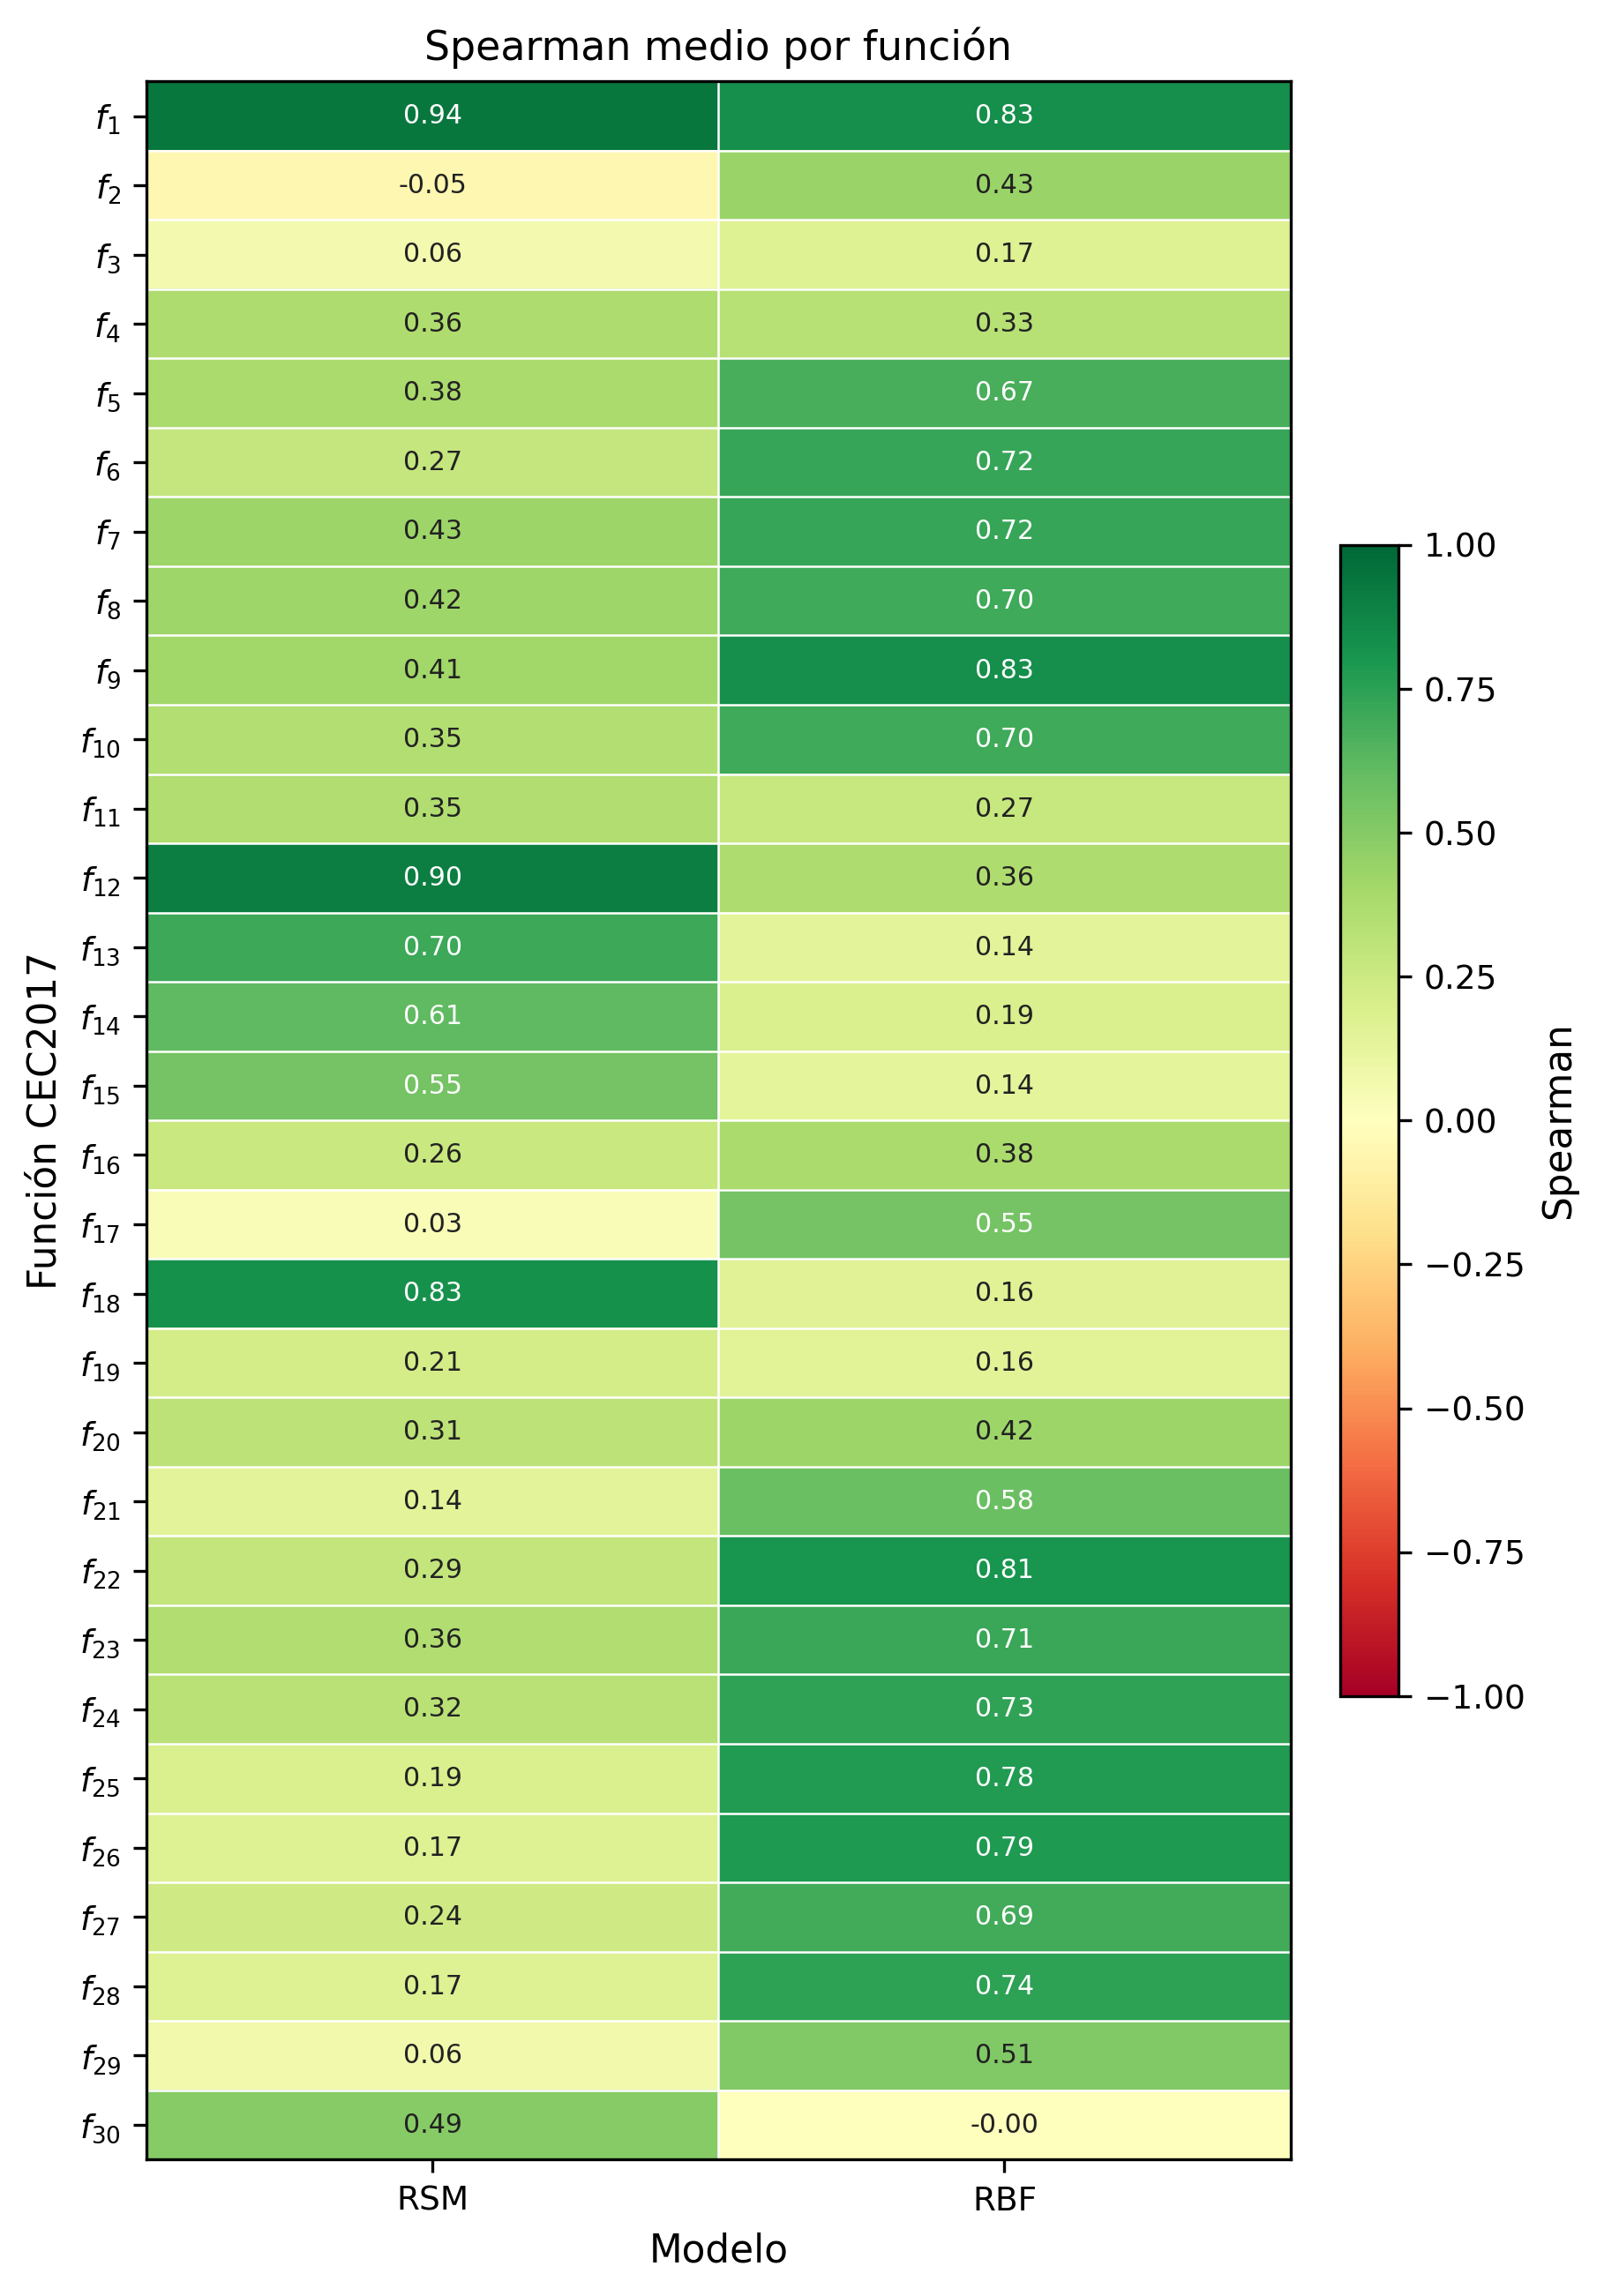
\includegraphics[width=1\textwidth]{figuras/surrogates_offline/heatmap_spearman_final_cec2017.png}
    \caption[Mapa de calor del coeficiente de correlación de Spearman medio por función y modelo]{Mapa de calor del coeficiente de correlación de Spearman medio por función y modelo. El valor anotado en cada celda corresponde al Spearman medio agregado sobre las semillas, los bloques de validación y las metaheurísticas consideradas.}
    \label{fig:heatmap_spearman_final_cec2017}
\end{figure}

A partir de esta figura se observa que ninguno de los dos modelos presenta un comportamiento uniforme en todo el benchmark. Sin embargo, RBF mantiene valores de correlación más estables en un mayor número de funciones, incluidas varias funciones híbridas y compuestas. RSM, por el contrario, concentra su rendimiento en funciones de baja complejidad y muestra una degradación más acusada en problemas de mayor complejidad estructural.

No obstante, los valores medios de nRMSE y nMAE de la
Tabla~\ref{tab:comparativa_configuraciones_ajustadas} resultan elevados en comparación con los observados durante el cribado. Para determinar si este comportamiento es general o está provocado por valores extremos (\textit{outliers}), la Figura~\ref{fig:boxplot_nrmse_final_cec2017} muestra la distribución de los errores en escala logarítmica y la Figura~\ref{fig:heatmap_nrmse_final_cec2017} localiza las funciones que concentran los valores más extremos (\textit{outliers}).

\begin{figure}[htbp]
    \centering
    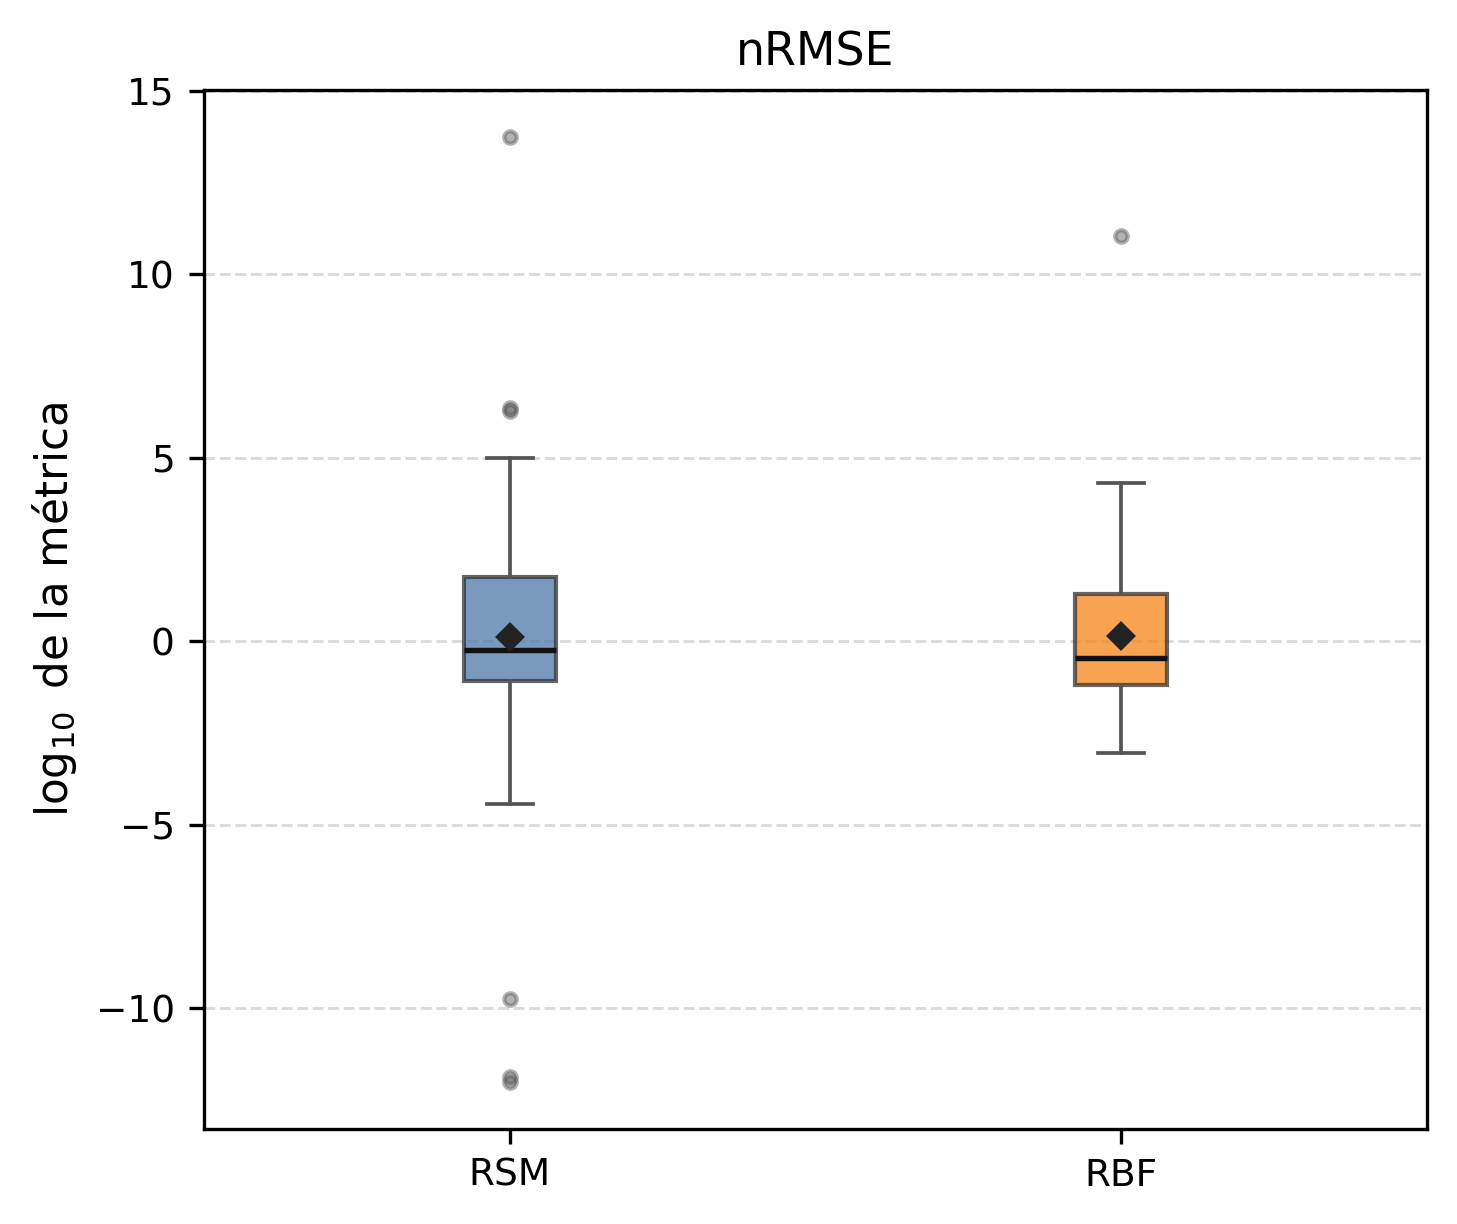
\includegraphics[width=0.9\textwidth]{figuras/surrogates_offline/boxplot_nrmse_final_cec2017.png}
    \caption{Distribución de nRMSE en escala logarítmica para las configuraciones finales de RSM y RBF sobre CEC2017 completa.}
    \label{fig:boxplot_nrmse_final_cec2017}
\end{figure}

\begin{figure}[htbp]
    \centering
    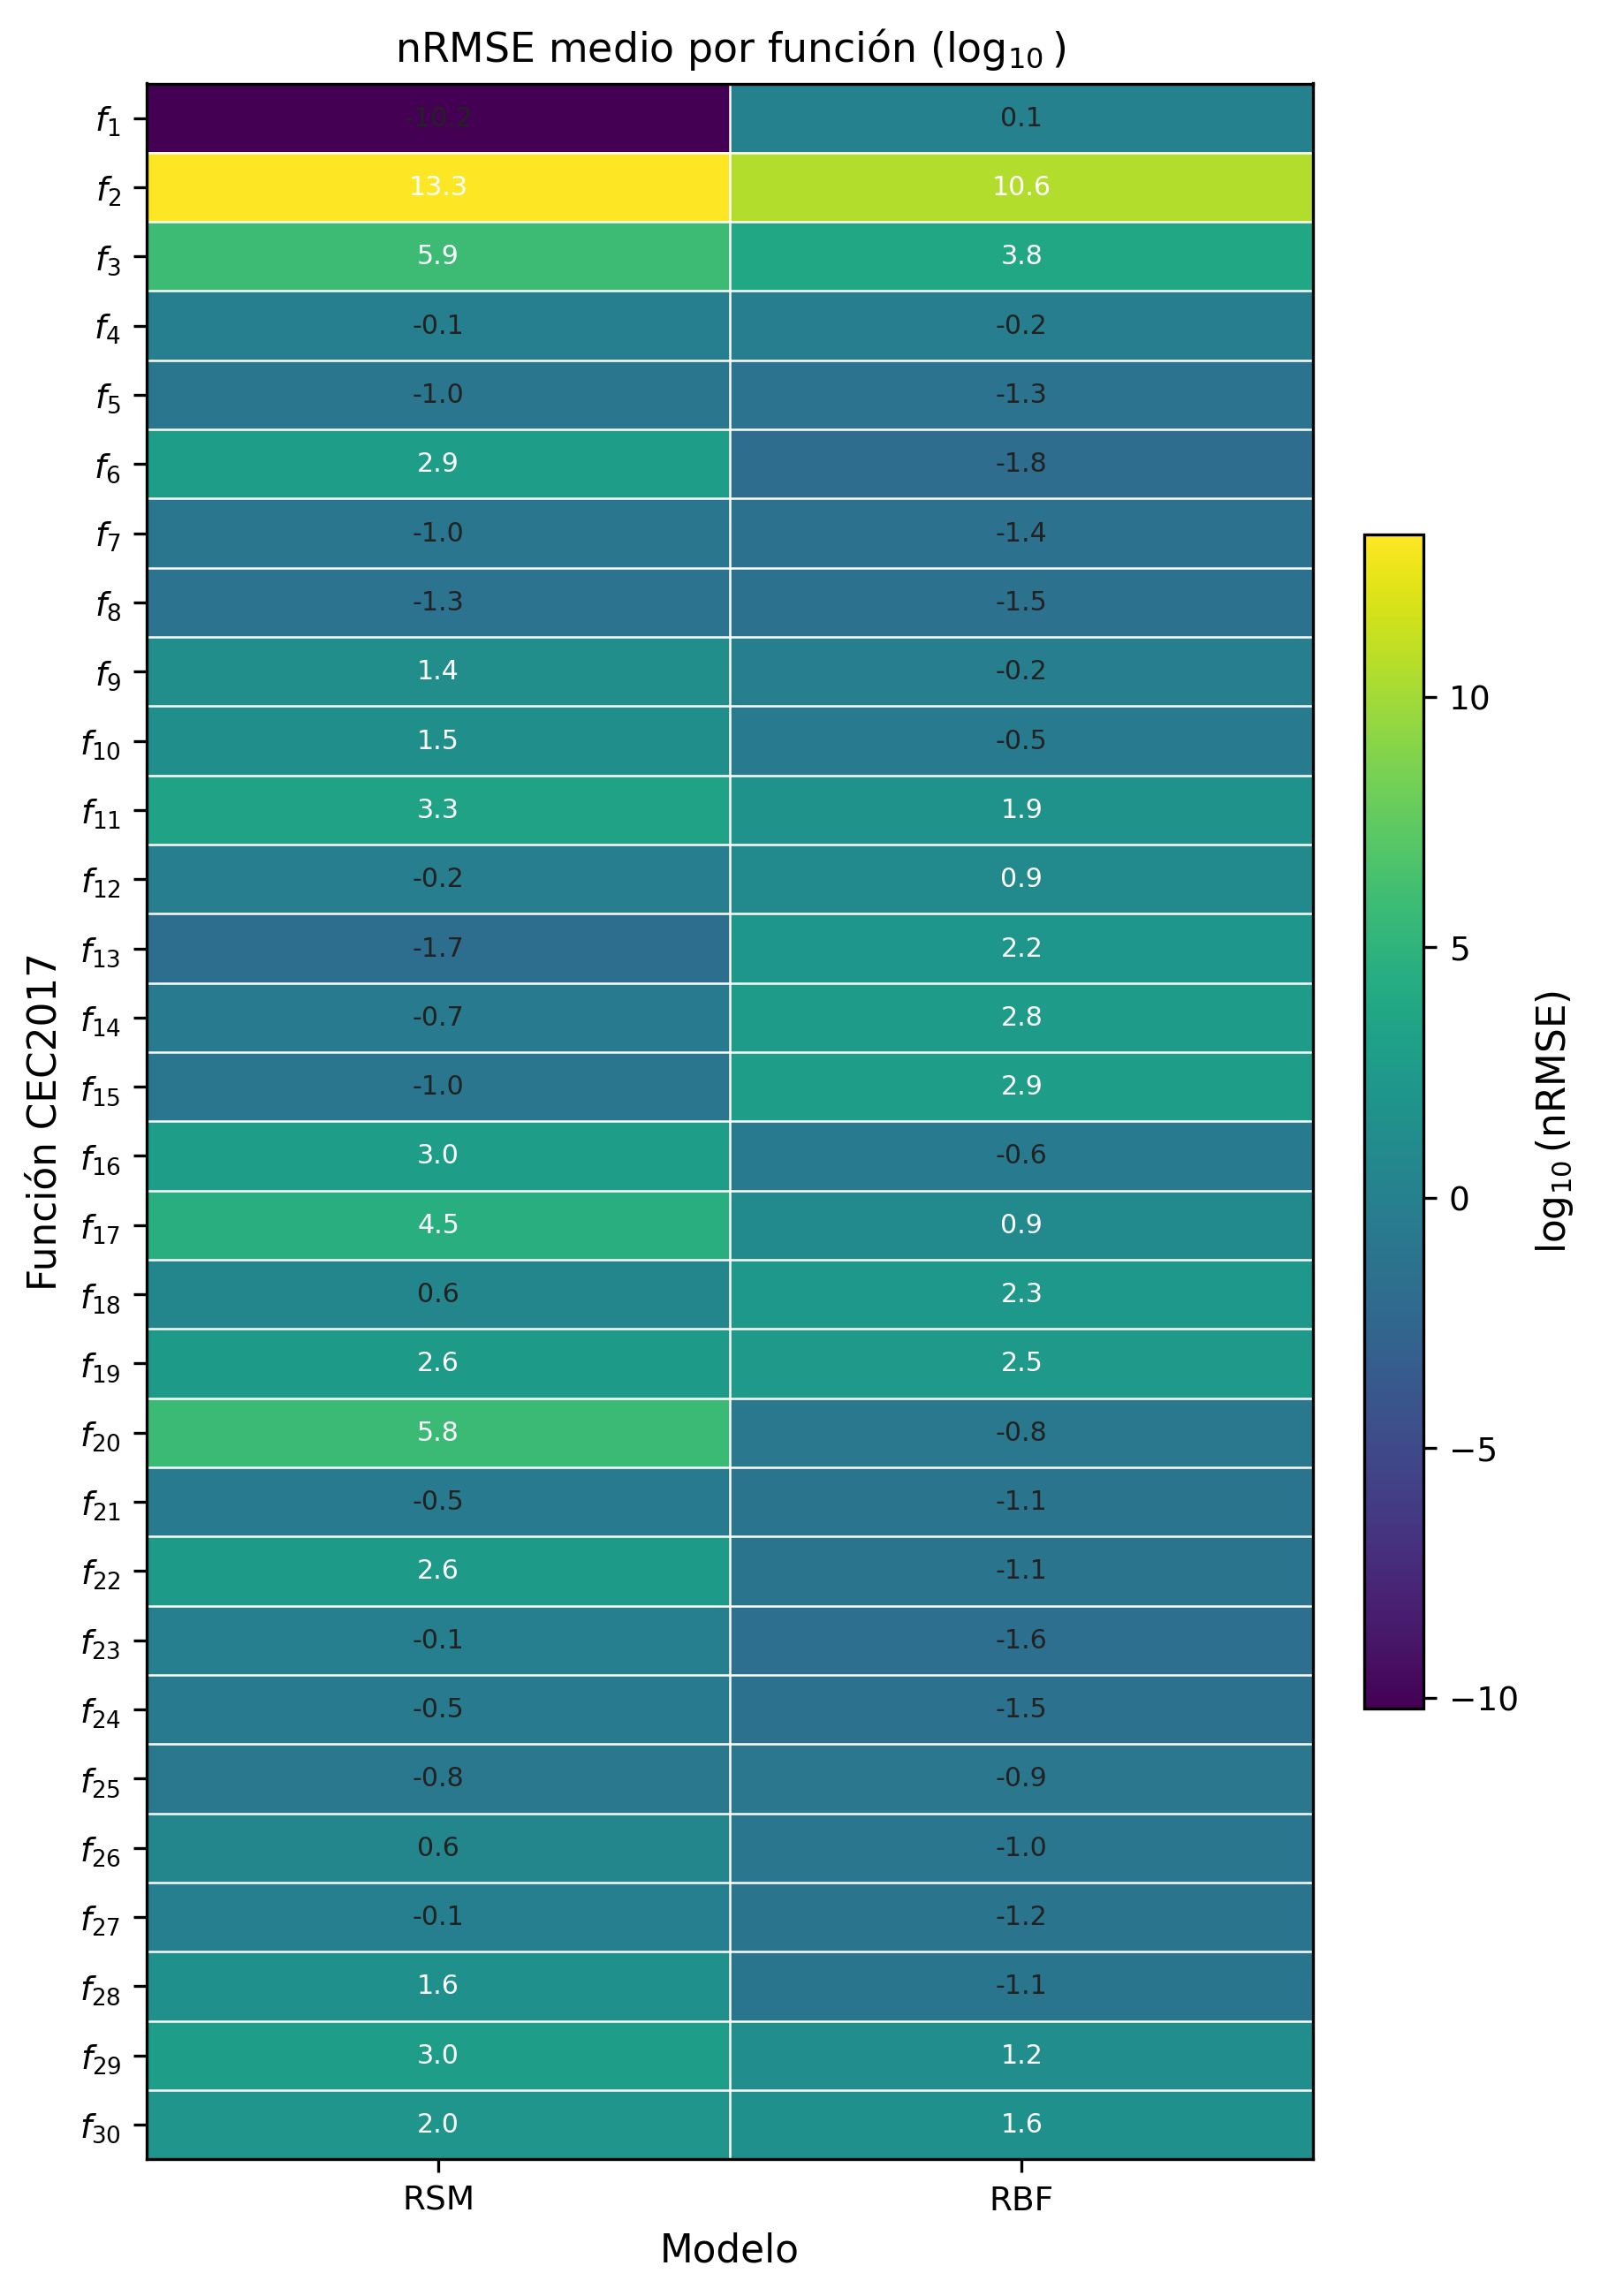
\includegraphics[width=1\textwidth]{figuras/surrogates_offline/heatmap_nrmse_final_cec2017.png}
    \caption{Mapa de calor del nRMSE medio por función y modelo en escala logarítmica.}
    \label{fig:heatmap_nrmse_final_cec2017}
\end{figure}

El \textit{boxplot} demuestra que la media está dominada por \textit{outliers}. La distribución para ambos modelos presenta colas pronunciadas mientras que la mediana se sitúa en rangos más moderados.

Por otro lado, el \textit{heatmap} identifica \(f_2\) como la principal responsable, cuyos valores de nRMSE superan en varios órdenes de magnitud al resto del benchmark en ambos modelos, especialemente para RSM, lo que justifica medias de error superiores. Este comportamiento es coherente con lo indicado en la Sección~\ref{subsec:suite_cec2017}, donde \(f_2\) fue excluida en revisiones posteriores de CEC2017 debido a sus inestabilidades numéricas. En este trabajo se mantiene para respetar la definición experimental del Capítulo~\ref{chap:metodologia_experimental}.

Teniendo en cuenta el análisis realizado, RBF muestra el comportamiento más
adecuado para continuar con la integración \textit{online}. Aunque sus errores
medios se ven afectados por valores extremos, especialmente en \(f_2\), el
modelo mantiene una mayor capacidad de ordenación que RSM sobre la suite
completa. Esta diferencia es especialmente relevante en el contexto de este
trabajo, ya que el objetivo del subrogado no es sustituir de forma exacta a la
función objetivo, sino apoyar la búsqueda preservando el orden relativo entre
soluciones candidatas. Además, su tiempo de entrenamiento es reducido, por lo
que el coste de reajustar el modelo durante la búsqueda no resulta
especialmente limitante. Su principal desventaja se encuentra en el tiempo de
predicción, superior al de RSM, aunque este incremento se considera asumible frente a la
mejora obtenida en la capacidad ordinal.

Este análisis permite extraer una conclusión más general sobre las técnicas
evaluadas, siempre dentro del escenario experimental considerado. Para las
trayectorias generadas sobre CEC2017 con dimensión \(D=10\) y tamaño de
población \(50\), una mayor complejidad del modelo no se traduce
necesariamente en una mejor utilidad como subrogado. En particular, los modelos
clásicos como RBF o RSM parecen adaptarse mejor al criterio principal de
evaluación con un coste computacional controlado, mientras que los modelos de
aprendizaje automático considerados, como los modelos basados en árboles o
redes neuronales, no alcanzan una mejora suficiente en Spearman como para
compensar su complejidad o su coste.

Por tanto, se selecciona \textbf{RBF} como el modelo subrogado para la
fase \textit{online}. RSM queda descartado como alternativa final pese a su bajo
tiempo de predicción, ya que su capacidad de ordenación es menor y su
comportamiento resulta menos estable al ampliar la evaluación al benchmark
completo.

\subsection{Validación del escenario de evaluación}

Tras seleccionar la mejor técnica subrogada sobre trayectorias con reinicio, se comprueba si la elección de un escenario sin reinicio conduciría a conclusiones diferentes o si, por el contrario, dichas trayectorias producen una evaluación menos informativa.

La Tabla~\ref{tab:comparativa_reinicio_surrogate} contrasta los resultados de RBF cuando las metaheurísticas operan con y sin reinicio.

\begin{table}[H]
    \centering
    \small
    \begin{adjustbox}{max width=\textwidth}
        \begin{tabular}{lccccc}
            \toprule
            \textbf{Escenario} & \textbf{Spearman} & \textbf{nRMSE}                  & \textbf{nMAE}                   & \textbf{Entren. (s)} & \textbf{Pred. (s)} \\
            \midrule
            Con reinicio       & \textbf{0.5074}   & \(\mathbf{1.2389 \times 10^9}\) & \(\mathbf{9.5968 \times 10^8}\) & 0.0057               & 0.7076             \\
            Sin reinicio       & 0.5023            & \(7.0201 \times 10^{10}\)       & \(5.1973 \times 10^{10}\)       & \textbf{0.0047}      & \textbf{0.3944}    \\
            \bottomrule
        \end{tabular}
    \end{adjustbox}
    \caption[Comparación de métricas de RBF con y sin reinicio de las metaheurísticas]{Comparación de métricas de RBF con y sin reinicio de las metaheurísticas. Medias calculadas sobre todas las funciones, semillas y bloques de validación.}
    \label{tab:comparativa_reinicio_surrogate}
\end{table}

Los resultados agregados muestran que el escenario con reinicio consigue una capacidad de ordenación ligeramente superior y reduce notablemente los errores medios normalizados respecto a las trayectorias sin reinicio. Aunque este último presenta menores tiempos de entrenamiento y predicción, esta reducción de coste no implica necesariamente una evaluación más adecuada del subrogado para la integración \textit{online}.

Como se demostró en la Sección \ref{sec:resultados_reinicio}, las trayectorias pueden quedar dominadas por fases prolongadas de estancamiento, en las que las muestras de validación presentan valores de \textit{fitness} muy similares entre sí. En esas condiciones, los errores normalizados pueden disminuir artificialmente sin que ello implique que el modelo haya aprendido una aproximación más útil para guiar la búsqueda.

Este efecto se aprecia con claridad en \(f_4\). La Tabla~\ref{tab:ejemplo_f4_sin_reinicio} muestra la evolución del
nMAE medio por bloque temporal para RBF sobre \(f_4\), comparando ambos
escenarios.

\begin{table}[H]
    \centering
    \small
    \begin{tabular}{lcc}
        \toprule
        \textbf{Bloque de entrenamiento} & \textbf{Con reinicio} & \textbf{Sin reinicio} \\
        \midrule
        1--20\%                          & 0.1295                & 0.1267                \\
        21--40\%                         & 0.1140                & 0.0012                \\
        41--60\%                         & 0.0414                & 0.0006                \\
        61--80\%                         & 0.0363                & 0.0004                \\
        \bottomrule
    \end{tabular}
    \caption{nMAE medio de RBF sobre \(f_4\) con y sin reinicio por bloque temporal.}
    \label{tab:ejemplo_f4_sin_reinicio}
\end{table}

En el primer bloque temporal, ambos escenarios presentan errores muy similares. Sin embargo, a partir del segundo bloque el error sin reinicio cae hasta valores prácticamente nulos, mientras que el escenario con reinicio mantiene errores mayores al conservar una trayectoria más variable.

No obstante, este comportamiento no indica que el subrogado haya aprendido una aproximación más útil de la función objetivo, sino que la trayectoria ha alcanzado una región de estancamiento total. En este contexto, las muestras del bloque futuro presentan valores de \textit{fitness} muy próximos, por lo que la tarea de predicción pierde el sentido.

Por tanto, las trayectorias con reinicio constituyen un escenario de evaluación
más exigente y más representativo para el objetivo de este trabajo. Al reactivar
la búsqueda, el reinicio mantiene una mayor variabilidad en las muestras
generadas y evita que la evaluación del subrogado quede condicionada por tramos estancados. En consecuencia, la selección de RBF sobre el
escenario con reinicio se considera metodológicamente más fiable para estudiar
su posterior integración \textit{online}.


\section{Evaluación de la estrategia \textit{online}}
\label{sec:online}

La última fase experimental estudia la integración \textit{online} del modelo \textbf{RBF} seleccionado en las secciones anteriores. Siguiendo el protocolo definido en la Sección~\ref{sec:diseno_online}, primero se calibran los parámetros específicos de la hibridación y, posteriormente, se evalúa su efecto sobre las metaheurísticas consideradas en el escenario con reinicio fijado previamente. El objetivo es comprobar si el filtro subrogado aporta una mejora real frente a la misma metaheurística sin intervención subrogada y si el coste añadido por su
uso resulta asumible.

\subsection{Calibración de los parámetros de integración}

%% no repetimos la definicion de los parámetros. 

En coherencia con los resultados obtenidos en la evaluación \textit{offline}, el subrogado se actualiza utilizando la
información más reciente disponible durante la ejecución.

A partir del protocolo descrito en la Sección~\ref{sec:diseno_online}, se evalúan los valores candidatos de cada parámetro sobre el subconjunto de funciones y semillas definido.

% - piloto de cooldown ya que depende del reinicio
% - piloto de retrain_ratio, porque controla actualizacion/coste del modelo
% - piloto de p, porque regula la agresivididad real del filtro y es el mas importante


% Los resultados muestran que cooldown=x, retrain_ratio=x y p=x ofrecen el mejor compromiso entre error final, ranking medio y coste computacional, por lo que se adoptan como configuración final para la evaluación online completa.

\subsection{Resultados frente a la metaheurística sin filtro}

%%%%%%%%%%%%%%%%%%%%%%%%%%%%%%%%%%%%%%%%%%%%%%%%%%%%%%%%%%%%
%%%%%%%%%%%%%%%%%%%%%%%%%%%%%%%%%%%%%%%%%%%%%%%%%%%%%%%%%%%%
%% resultado importante del trabajo

% - configuración online final seleccionada
% - evaluacion final sobre 30 funciones y 51 semillasnuevas
% - comparacion p=0.00 vs p=0.50

%% el analisis debe responder "la intengracion online mejora realmente el prceso de optimización??"" y por ende, "comprobar si la version mh + subrogado mejora a la version original de cada mh".

%% en ningun momento estamos comparando los evolutivos con el estacionario -> NO NOS IMPORTA PARA NADA. solo nos importa que mejore la hibridacion -> si uno mejora, pues este MEJORA MUCHO y este NO MEJORA TANTO pero YA ESTA.

%% a lo mejor NO MEJORA pero lo que si vamos a ver al 100%, como poco, es que en la curva de convergencia la velocidad si incrementa.
% - esta no mejoria puede deberse a que reinicia demasiadas veces pero podemos justificarlo como: "se han aplicado tecnicas de reinicio pero realmente, si no tuvieramos ese reinicio y nos estabilizasemos cuando ya el algoritmo no mejora mas, estariamos parando MUCHO ANTES que DESPUES --> asi podemos venderlo

% esta claro que si la MH SE ESTANCA, no tiene sentido el papel e integración de los subrogados -> o paramos o aplicamos reinicio


% - Evaluación del ahorro de evaluaciones reales.
% - convergencia
% - Discusión de cuándo ayuda y cuándo perjudica.
%%%%%%%%%%%%%%%%%%%%%%%%%%%%%%%%%%%%%%%%%%%%%%%%%%%%%%%%%%%%
%%%%%%%%%%%%%%%%%%%%%%%%%%%%%%%%%%%%%%%%%%%%%%%%%%%%%%%%%%%%
% - tabla principal
% - analisis
% - parrafo de diagnostico: porcentaje de rechazo, numero de entrenamieto, tiempo online, si el filtro esta siendo demsaido agresivo o razonable...

% ejemplo: Además del error final, los contadores de la integración permiten interpretar el efecto del filtro. En las ejecuciones con \(p=0.50\), el subrogado no reduce el presupuesto total de evaluaciones reales, que se mantiene fijo, sino quedescarta candidatos antes de su evaluación y desplaza el presupuesto hacia otros candidatos generados posteriormente. Por tanto, el porcentaje de rechazo y el tiempo dedicado al modelo permiten valorar si la mejora obtenida compensa la intervención del filtro.

% - Si mejora el error final y rechaza muchos candidatos: el filtro está funcionando bien.
% - Si empeora y rechaza muchos candidatos: probablemente está descartando candidatos útiles.
% - Si apenas rechaza candidatos: el subrogado interviene poco y su impacto será limitado.
% - Si el tiempo online sube mucho: aunque mejore algo, puede no compensar.
%%%%%%%%%%%%%%%%%%%%%%%%%%%%%%%%%%%%%%%%%%%%%%%%%%%%%%%%%%%%
%%%%%%%%%%%%%%%%%%%%%%%%%%%%%%%%%%%%%%%%%%%%%%%%%%%%%%%%%%%%



%% criterio de reinicio - cooldown

% por la definicion de criterio de reactivacion que se ha definido y por los resultados obtenidos en este mismo capitulo cuando hablamos de la motivacion del reinciio y analizamos graficas tras aplicarlo posteriromente, se podia ver que la poblacion cambiaba bruscamente, por ese motivo, se considera evaluar..

% Si el subrogado se usa inmediatamente, puede estar entrenado sobre una distribución que ya no representa la nueva población.

% Por ello se introduce un periodo de enfriamiento o cooldown, durante el cual se priorizan evaluaciones reales antes de volver a confiar en el modelo.

% La inclusión de un periodo de enfriamiento tras el reinicio se justifica tanto
% por la definición del propio mecanismo como por el comportamiento observado en
% los experimentos anteriores. El reinicio elitista conserva únicamente la mejor
% solución encontrada y regenera el resto de la población, por lo que introduce un
% cambio abrupto en la distribución de candidatos disponibles. Este efecto ya se
% aprecia en el análisis del reinicio realizado al comienzo de este capítulo,
% donde la reactivación de la población modifica la dinámica de convergencia y de
% diversidad. En consecuencia, utilizar inmediatamente un subrogado entrenado con
% muestras anteriores al reinicio podría conducir a predicciones poco
% representativas. Por este motivo, se incorpora como parámetro experimental un
% periodo de enfriamiento durante el cual se retrasa el uso del subrogado y se
% prioriza la generación de nuevas evaluaciones reales.

% La conclusión clara es que la hibridación con p=0.50 no mejora de forma homogénea a las tres metaheurísticas. Funciona mejor en DE, no compensa en AGE y queda muy cerca de neutra en SHADE.

% Para AGE, el filtro rechaza bastantes candidatos, alrededor del 64.7%, pero el rendimiento final empeora. Eso apunta a que el subrogado está interviniendo de forma efectiva, pero no de forma beneficiosa: probablemente descarta candidatos que sí podían ser útiles para la dinámica estacionaria de AGE.

% Para DE, el resultado es el más favorable. p=0.50 gana muchas más veces de las que pierde y mejora el ranking medio. Aun así, hay que matizar que la media empeora por funciones con outliers, especialmente en funciones compuestas como f30. Por eso, para DE la lectura correcta es: mejora robusta en términos pareados/ranking/mediana, pero con coste computacional alto y sensibilidad en algunos casos.

% Para SHADE, no hay una mejora suficientemente clara. El ranking medio queda casi empatado y las pérdidas superan ligeramente a las mejoras. Aquí el filtro interviene mucho, con rechazo cercano al 74%, pero no se traduce en una mejora final estable.

% De cara a la memoria, yo lo redactaría así: la configuración p=0.50 seleccionada en pilotos muestra que la integración online puede aportar valor, pero su efecto depende de la metaheurística. La evidencia más favorable aparece en DE; en AGE resulta perjudicial y en SHADE no ofrece una ventaja clara. Esto es una conclusión fuerte y honesta para la sección final online.


% El piloto de enfriamiento tras reinicio muestra que introducir una pausa después del reinicio resulta beneficioso frente a activar el filtro inmediatamente. Entre los valores evaluados, \(100\) evaluaciones ofrece el mejor compromiso agregado: obtiene el mejor ranking medio en AGE, DE y SHADE y concentra el mayor número de funciones ganadas. Valores menores parecen insuficientes para estabilizar la nueva región explorada, mientras que valores mayores retrasan en exceso la intervención del subrogado


% La calibración se realiza de forma secuencial, no como una búsqueda exhaustiva sobre todas las combinaciones posibles. Por tanto, los valores seleccionados no deben interpretarse como óptimos globales, sino como una configuración homogénea y computacionalmente viable para evaluar la integración online en las tres metaheurísticas.

% El valor de enfriamiento se estudia manteniendo fijos el resto de parámetros de integración. Bajo esta configuración de referencia, \(100\) evaluaciones proporciona el mejor comportamiento agregado, por lo que se adopta como valor base para los pilotos posteriores.

\subsection{Comparación con técnicas subrogadas de referencia}

% - comparacion con técnicas de referencia como kriging y pce

%%%%%%%%%%%%%%%%%%%%%%%%%%%%%%%%%%%%%%%%%%%%%%%%%%%%%%%%%%%%
%%%%%%%%%%%%%%%%%%%%%%%%%%%%%%%%%%%%%%%%%%%%%%%%%%%%%%%%%%%%
%% comparación breve

%% rbf online, kriging online, pce online y p=0 como referencia.
%% no haremos una discusion larga modelo a modelo. el objetivo es comprobar si RBF, elegido mediante la fase offline y ya demostrado su mejor rendimiento frente a modelos de aprendizaje automatico mas complejos tratados como subrogados, tambn es competitivo frente a técnicas clasicas en integracion real --> tenemos un algoritmo que es mas complejo y no es necesario ya que tenemos una tecnica matematica que va mejor, por ejemplo.
%%%%%%%%%%%%%%%%%%%%%%%%%%%%%%%%%%%%%%%%%%%%%%%%%%%%%%%%%%%%
%%%%%%%%%%%%%%%%%%%%%%%%%%%%%%%%%%%%%%%%%%%%%%%%%%%%%%%%%%%%
\subsection{Conclusiones de la integración \textit{online}}


%% cerrar brevemente con varias ideas:

%% si la hibridacion mejora o no mejora frente a la metaheuristica base
%% si el coste añadido es razonable
%% si el filtro es lo suficientemente robusto para las metaheuristicas consideradas o si su utilidad depende del algoritmo.










% Por qué el Spearman alto sin reinicio es engañoso:

% Cuando la metaheurística se estanca, la población converge a una región pequeña del espacio. Los valores de fitness de soluciones vecinas son muy similares y localmente suaves. Predecir el orden relativo de
% puntos casi idénticos es un problema trivial para cualquier modelo — el Spearman sube porque la tarea es más fácil, no porque el subrogado sea más útil.

% La evidencia más clara la tienes en las medianas de nRMSE: 0.0004 sin reinicio frente a 0.8389 con reinicio en las mismas funciones. Esa diferencia de tres órdenes de magnitud en el error típico es
% precisamente la huella de ese efecto: sin reinicio, los valores de fitness son tan parecidos entre sí que los errores absolutos son mínimos.


% El punto clave para tu TFG:

% El escenario relevante para la integración online es el de trayectorias dinámicas — con reinicios, cambios de región y alta diversidad de muestras. Evaluar el subrogado sobre trayectorias estancadas produce
% una estimación optimista que no se corresponde con el contexto real de uso. Por tanto, comparar ambos escenarios para elegir el modelo sería metodológicamente incorrecto.

% Una matiz que conviene tener presente:

% La diferencia en Spearman entre escenarios no es dramática (0.80 vs 0.74 en mediana), lo que refuerza el argumento: el subrogado no "pierde" capacidad porque hay reinicio, sino que se enfrenta a un problema
% más exigente y realista. Eso es lo que hay que transmitir en el texto si decides incluir esta comparación.